%!TEX TS-program = pdflatex
\documentclass{robinthesisdraft}
\def\pgfsysdriver{pgfsys-pdftex.def}
\usepackage{robincs,thesisdefs,xr,tikz,prooftree}
\externaldocument[Bicats:]{bicats}
\externaldocument[MonBicats:]{mon-bicats}
\tikzstyle{every picture}+=[remember picture, >=latex]

\title{A Language for Monoidal Bicategories}
\begin{document}
\maketitle
%
\section{The problem}
Even with the help of the coherence theorem, it can be extremely
tedious to prove even simple facts about pseudomonoids. The problem
is essentially notational rather than mathematical: in an ordinary
category, we can use commutative diagrams to establish equations
between arrows. It is almost always easier to understand a diagram
than an explicit sequence of equalities between expressions, because
\begin{itemize}
\item The types of the arrows are clear from the diagram.
\item The diagram abstracts away from certain details of the proof:
	if two equations could be applied in either order, the diagram
	does not have to choose an order arbitrarily.
\item The global structure of the whole argument can be seen at a glance.
\end{itemize}
In a bicategory, to prove an equation between 2-cells by similar
means, we should need three-dimensional diagrams. This poses
practical problems -- paper is two-dimensional -- and also requires
the reader to visualise a three-dimensional structure, something
that most humans do not find easy. This technique has sometimes
been attempted nonetheless: by \citet[][Section~3.4]{LackThesis},
for example.
%
The more usual alternative is to use a sequence of equations
between string or pasting diagrams. As well as using a lot
of paper, such proofs are often difficult to follow.
% XXXX - is the following still true??
(We do find ourselves obliged to resort to this technique in some
places where the techniques of this chapter do not apply.)

The purpose of this chapter is to show how these notational
difficulties may, in some cases, be overcome by using a formal
language to specify 1-cells, 2-cells, and equations between 2-cells
in a monoidal bicategory. The syntax of the language is designed in such
a way that a proof using the language closely resembles -- typically,
is formally identical to -- a proof
using categories, functors and natural transformations in the usual
way. In other words, provided that one uses only admissible techniques,
a proof in the 2-monoidal 2-category $\Cat$ may be reinterpreted
as a general proof that applies to any monoidal bicategory. In particular,
we shall be able to prove various general facts about pseudomonoids
simply by reusing the usual proof of the corresponding fact for
monoidal categories. The language could be regarded as a higher-dimensional analogue
of the formal language developed \citet{JayLanguages} for monoidal
categories.

This formal language is not completely general. The fundamental
restriction is that it may only be used to talk about theories
whose 1-cells are of the form
\[
	A_{1}\tn\cdots\tn A_{n} \to B.
\]
In particular, the braiding on a braided Gray monoid is not of this
form, and we will need an extension of the language to prove facts about
structures that interact with the braiding, such as the braiding of
a braided pseudomonoid. This extended language is developed in
the next chapter.
% %
% This restriction could probably be weakened to some extent, but
% only by compromising the simplicity of the language.

Most of the formal development is fairly routine. The interpretation of
a theory is defined first for Gray monoids, and then extended to arbitrary
monoidal bicategories using coherence. The only technically difficult part
is to account for the non-strictness of the interchange law in a Gray monoid,
which requires some detailed technical work (\ref{s-semantics-of-substitution}
and~\ref{s-interpretation-of-2-cells}).

\section{The language}
The language is used to prove equations between 2-cells that hold in
every model of a given theory.
%
We require the theory to be presented as a collection
of objects, (multi-)1-cells, 2-cells and equations between 2-cells.

A \emph{theory} $\T$ consists of:
\begin{itemize}
	\item A set $\T_{0}$ of \emph{objects},
	\item For every non-empty sequence $\A_{1}, \ldots, \A_{n}, \CB$ of
		elements of $T_{0}$,
		a set $\T(\A_{1},\ldots,\A_{n};\CB)$
		of \emph{1-cells} $(\A_{1}, \dots, \A_{n})\to \CB$.
		We suppose that the different sets of 1-cells are pairwise disjoint.
	\item Sets of 2-cells and equations, as described below.
\end{itemize}
Before we attempt a formal description of the 2-cells and equations,
we shall introduce the part of the language that describes 1-cells.

\subsection{1-cells}
A 1-cell will be described by a \emph{1-cell sequent}: suppose
we are considering a theory with objects $\A, \CB, \C$ and
1-cells $f: (\A,\CB)\to\C$ and $g:\C\to\C$. Then the arrow
\[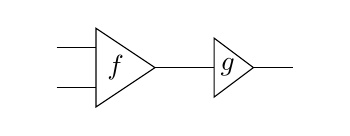
\begin{tikzpicture}[scale=0.25]
	\draw (0,-2) -- (0,2) -- (3,0) -- cycle ;
		\node at (1,0) {$f$} ;
	\node at (-3,1)  {$\A$}  ; \draw (-2,1) -- (0,1) ;
	\node at (-3,-1) {$\CB$} ; \draw (-2,-1) -- (0,-1) ;
	\draw (3,0) -- (6,0)
		node[pos=0.5,auto] {$\C$} ;
	\draw (6,-1.5) -- (6,1.5) -- (8,0) -- cycle ;
		\node at (6.7,0) {$g$} ;
	\draw (8,0) -- (10,0) ;
		\node at (11,0) {$\D$} ;
\end{tikzpicture}\]
might be represented by the sequent
\[
	A\in\A, B\in\CB \proves g(f(A,B)) \in \D.
\]
The names in the context -- to the left of the turnstile -- should
be regarded as bound, so for example the sequent
\[
	X\in\A, Y\in\CB \proves g(f(X,Y)) \in \D
\]
is equivalent to the one above, modulo the renaming of bound
variables, and represents the same 1-cell. (We assume
throughout that we have some infinite set of names
on which to draw. Names here will be represented
by upper-case italic letters.)
Formally, the derivation rules for 1-cell sequents are
as follows:
\begin{itemize}
\item The axiom rule: for every $\C\in\T_{0}$,
\[
	\begin{prooftree}
		\justifies A\in\C \proves A\in\C \using (\C)
	\end{prooftree}
\]
\item The application rule: for every $f\in\T(\A_{1},\dots,\A_{n}; \CB)$,
\[
	\begin{prooftree}
		\Gamma_{1}\proves \alpha_{1}\in \A_{1}
		\quad
		\cdots
		\quad
		\Gamma_{n}\proves \alpha_{n}\in \A_{n}
		\justifies
		\Gamma_{1},\dots,\Gamma_{n} \proves f(\alpha_{1},\dots,\alpha_{n})\in\CB
		\using f(\bullet)
	\end{prooftree}
\]
where the sets of names in the $\Gamma_{i}$ are assumed pairwise disjoint.
\end{itemize}
(Whenever several contexts are mentioned together, we shall \emph{always} assume
that their sets of names are pairwise disjoint, usually without explicitly mentioning
this assumption.)
So a 1-cell sequent is simply a formal composite of formal 1-cells.
It is clear (and easily proved by induction) that every derivable 1-cell
sequent has a unique derivation. Also:
\begin{definition}
	Let $A_{1}\in\A_{1}, \cdots, A_{n}\in\A_{n}\proves \beta\in\CB$
	be a derivable 1-cell sequent; and for every $1\leq i\leq n$, let
	$\Gamma_{i} \proves \alpha_{i}\in\A_{i}$ be a derivable 1-cell sequent.
	Then we write $[A_{i} := \alpha_{i}]_{i=1}^{n}$ to denote the multiple
	substitution
	\[
		[A_{1} := \alpha_{1}, \cdots, A_{n}:= \alpha_{n}].
	\]
	On occasion this is abbreviated to $[A_{i} := \alpha_{i}]_{i}$,
	where the value of $n$ is apparent from the context.
	
	Later, we sometimes need to use nested sequences: if
	\[
		(A^{1}_{1}, \cdots, A^{1}_{n_{i}}),
		\dots,
		(A^{n}_{1}, \cdots, A^{n}_{n_{n}})
	\]
	is a nested sequence of objects, with $\alpha^{i}_{j}$ being
	a similarly-numbered nested sequence of 1-cell expressions, then
	\[
		[[A^{i}_{j} := \alpha^{i}_{j}]_{j=1}^{n_{i}}]_{i=1}^{n}
	\]
	denotes the substitution
	\[
		[A^{1}_{1} := \alpha^{1}_{1}, \cdots, A^{1}_{n_{1}}:= \alpha^{1}_{n_{1}},
		\enskip\cdots,\enskip
		A^{n}_{1} := \alpha^{n}_{1}, \cdots, A^{n}_{n_{n}}:= \alpha^{n}_{n_{n}}
		].
	\]
\end{definition}
\begin{lemma}[1-cell substitution]
	If $A_{1}\in\A_{1}, \cdots, A_{n}\in\A_{n}\proves \beta\in\CB$
	is a derivable 1-cell sequent, and for every $1\leq i\leq n$,
	$\Gamma_{i} \proves \alpha_{i}\in\A_{i}$ is a derivable 1-cell sequent,
	with the names in the $\Gamma_{i}$ pairwise disjoint, then
	\[
		\Gamma_{i},\cdots,\Gamma_{n}\proves \beta[A_{i} := \alpha_{i}]_{i=1}^{n}
	\]
	is a derivable 1-cell sequent,
\end{lemma}
\begin{proof}
	Consider a derivation of $\beta$, and make the substitution
	throughout the derivation, as follows. For each sequent
	$\Gamma\proves \gamma\in\C$ in the derivation, replace $\gamma$
	by $\gamma[A_{i} := \alpha_{i}]_{i}$, and replace each name
	$A_{i}\in\A_{i}$ of $\Gamma$ by the contents of $\Gamma_{i}$.
	%
	Each application rule is thus transformed
	into another instance of that application rule, and each axiom
	$A_{i}\in\A_{i} \proves A_{i}\in\A_{i}$
	is transformed into $\Gamma_{i}\proves \alpha_{i}\in\A_{i}$, which is
	derivable by assumption.
\end{proof}

\subsection{2-cells}
Now we can define the 2-cells of $\T$. In addition to the
objects and 1-cells, we have:
for every pair $\Gamma\proves\alpha\in\CB$, $\Gamma\proves\beta\in\CB$
of derivable 1-cell sequents, a set $\T^{\Gamma}_{\CB}[\alpha,\beta]$
of 2-cells. Of course, we take these to be invariant under renaming,
so if $\sigma$ is a permutation of the set of names then we require
\[
	\T^{\Gamma^{\sigma}}_{\CB}[\alpha^{\sigma},\beta^{\sigma}] = \T^{\Gamma}_{\CB}[\alpha,\beta].
\]
Any two \emph{different} sets of 2-cells (i.e.\ sets that are not presumed equal by the above)
are taken to be disjoint.
%
A 2-cell sequent is of the form $\Gamma\proves \phi: \alpha\to\beta \in\CB$.
The derivation rules for 2-cell sequents are:
\begin{itemize}
\item The identity rule:
	\[\begin{prooftree}
		\Gamma\proves \alpha\in\A
		\justifies
		\Gamma\proves 1_{\alpha}: \alpha\to\alpha\in\A
		\using 1
	\end{prooftree}\]
\item The axiom rule: for every $t\in \T^{\Gamma}_{\CB}[\alpha,\beta]$,
	with $\Gamma = (A_{1}\in\A_{1}, \dots, A_{n}\in\A_{n})$,
	\[\begin{prooftree}
		\Gamma_{1}\proves\gamma_{1}\in\A_{1}
		\quad\cdots\quad
		\Gamma_{n}\proves\gamma_{n}\in\A_{n}
		\justifies
		\Gamma_{1}\cdots\Gamma_{n} \proves t_{\gamma_{1},\dots, \gamma_{n}}
			: \alpha[A_{i} := \gamma_{i}]_{i}
			\to\beta[A_{i} := \gamma_{i}]_{i}
			\in \CB
		\using t_{\bullet} 
	\end{prooftree}\]
	where the sets of names in the $\Gamma_{i}$ are pairwise disjoint.
\item The composition rule:
\[\begin{prooftree}
	\Gamma\proves \phi: \beta\to\gamma \in\A
	\quad
	\Gamma\proves \psi: \alpha\to\beta \in\A
	\justifies
	\Gamma\proves \phi\cdot\psi: \alpha\to\gamma \in\A
	\using \mathrm{comp}
\end{prooftree}\]
\item The 1-cell application rule: for every $f\in\T(\A_{1},\dots,\A_{n};\CB)$,
	\[\begin{prooftree}
		\Gamma_{1}\proves \phi_{1} : \alpha_{1}\to\beta_{1} \in \A_{1}
		\quad \cdots \quad
		\Gamma_{n}\proves \phi_{n} : \alpha_{n}\to\beta_{n} \in \A_{n}
		\justifies
		\Gamma_{1},\cdots,\Gamma_{n}\proves f(\phi_{1},\dots,\phi_{n})
			: f(\alpha_{1},\dots,\alpha_{n}) \to f(\beta_{1},\dots,\beta_{n})
			\in\CB
		\using f(\to)
	\end{prooftree}\]
	The names in the $\Gamma_{i}$ are again required to be pairwise disjoint.
\end{itemize}
Since the conclusion of each rule has a distinct syntactic form, each derivable
2-cell sequent has a unique derivation.
Notice that, if $\Gamma\proves \phi:\alpha\to\beta\in\CB$ is a derivable
2-cell sequent, then $\Gamma\proves\alpha\in\CB$ and $\Gamma\proves\beta\in\CB$
are derivable 1-cell sequents.
%
We also observe that substituting a 1-cell expression in a 2-cell expression,
or vice versa, results in a derivable 2-cell sequent:
\begin{lemma}[1-in-2 substitution]\label{lemma-1in2}
	Let \( \Delta \proves \phi:\alpha\to\beta \in\C \)
	be a derivable 2-cell sequent, with
	\[
		\Delta = B_{1}\in\CB_{1}, \cdots, B_{n}\in\CB_{n}.
	\]
	For each $1\leq i\leq n$, let
	\[
		\Gamma_{i} \proves \gamma_{i}\in\CB_{i}
	\]
	be a derivable 1-cell sequent. Then the 2-cell sequent
	\[ \Gamma_{1}, \cdots, \Gamma_{n}
		\proves \phi[B_{i}:=\gamma_{i}]_{i}
		: \alpha[B_{i}:=\gamma_{i}]_{i}\to\beta[B_{i}:=\gamma_{i}]_{i}
		\in \C, \]
	is also derivable,
	assuming that the sets of names in the $\Gamma_{i}$ and $\Delta$
	are pairwise disjoint.
\end{lemma}
\begin{proof}
	Consider a derivation of \( \Delta \proves \phi:\alpha\to\beta \in\C \),
	and make the substitution throughout the derivation. In detail: for
	every sequent in the derivation, in the context replace each $B_{i}\in\CB_{i}$
	by $\Gamma_{i}$ and in the expression replace each $B_{i}$ by $\gamma_{i}$.
	For each derivation rule, this
	substitution results in another instance of the same rule, and the
	1-cell substitution lemma ensures that every 1-cell sequent in the
	derivation remains derivable. The conclusion of this new derivation
	is
	\[ \Gamma_{1}, \cdots, \Gamma_{n}
		\proves \phi[B_{i}:=\gamma_{i}]_{i}
		: \alpha[B_{i}:=\gamma_{i}]_{i}\to\beta[B_{i}:=\gamma_{i}]_{i}
		\in \C, \]
	which is therefore derivable.
\end{proof}
\begin{lemma}[2-in-1 substitution]\label{lemma-2in1}
	Let $\Gamma\proves\gamma\in\C$ be a derivable 1-cell sequent, for
	some \[ \Gamma = (A_{1}\in\A_{1},\dots, A_{n}\in\A_{n}). \]
	If the 2-cell sequents
	\[
	\Delta_{1}\proves \phi_{1} : \alpha_{1}\to\beta_{1} \in \A_{1}
	\quad \cdots \quad
	\Delta_{n}\proves \phi_{n} : \alpha_{n}\to\beta_{n} \in \A_{n}
	\]
	are all derivable, then so is
	\[
	\Delta_{1},\cdots,\Delta_{n}\proves \gamma[A_{i} := \phi_{i}]_{i}
		: \gamma[A_{i} := \alpha_{i}]_{i} \to \gamma[A_{i} := \beta_{i}]_{i}
		\in\CB.
	\]
	The names in the $\Delta_{i}$ must be pairwise disjoint, of course.
\end{lemma}
\begin{proof}
	\def\<#1>{\langle#1\rangle}
	This is simply a matter of repeatedly applying the 1-cell application
	rule. Formally,
	the proof is by induction on $\gamma$.
	If $\gamma$ is a constant, i.e.\ $\Gamma$ is the singleton $C\in\C$ and $\gamma$
	is just $C$, then the conclusion is equal to the hypothesis and the claim
	is trivial. Suppose, then, that $\gamma = f(\gamma_{1}, \dots, \gamma_{m})$ for some
	$m\in\N$, 1-cell symbol $f\in\T(\CB_{1}, \dots, \CB_{m}; \C)$ and
	1-cell expressions $\gamma_{i}$.
	
	Clearly the context $\Gamma$ must be equal to
	$(\Gamma_{1}, \cdots, \Gamma_{m})$, where each $\Gamma_{i}$ contains
	the names used in $\gamma_{i}$.
	%
	We want to reindex the names so that it is clear to which $\gamma_{i}$
	each belongs, for which we introduce a simple technical device that is
	also used in several other proofs below.
	For each $1\leq i\leq m$, let $m_{i}$ be the number of names in
	$\Gamma_{i}$. Then, given $1\leq i \leq m$ and $1\leq j\leq m_{i}$,
	define $\<i,j>$ to be $j+\sum_{r<i}m_{r}$. The effect of this definition
	is that
	\[
		\Gamma_{i} = (A_{\<i,1>} \in \A_{\<i,1>}, \cdots, A_{\<i,m_{i}>} \in \A_{\<i,m_{i}>})
	\]
	or, in abbreviated notation, that
	\[
		\Gamma_{i} = (A_{\<i,j>} \in \A_{\<i,j>})_{j=1}^{m_{i}}
	\]
	%
	The inductive hypothesis implies that, for each $1\leq i\leq m$, the
	2-cell sequent
	\[
	\Gamma_{i}\proves \gamma_{i}[A_{\<i,j>} := \phi_{\<i,j>}]_{j=1}^{m_{i}}
		: \gamma_{i}[A_{\<i,j>} := \alpha_{\<i,j>}]_{j=1}^{m_{i}}
		\to \gamma_{j}[A_{\<i,j>} := \beta_{\<i,j>}]_{j=1}^{m_{i}}
		\in\CB_{i}.
	\]
	is derivable. Now apply the 1-cell application rule to these sequents and
	the 1-cell symbol $f$, and the conclusion follows.
\end{proof}

\subsection{Equations}
The final ingredient that we need to complete our description
of $\T$ is a collection of equations between 2-cells.
Formally, we declare that for each pair
$\Gamma\proves\alpha\in\A$ and $\Gamma\proves\beta\in\A$ of
1-cell sequents, there is a set that we denote
$\T_{=}(\Gamma\proves \alpha\to\beta\in\A)$. This set consists
of pairs $(\phi,\psi)$,
where $\Gamma\proves\phi:\alpha\to\beta\in\A$ and
$\Gamma\proves\psi:\alpha\to\beta\in\A$ are derivable
2-cell sequents.
%
We also require the collection of equations to be closed under renaming,
so if $\sigma$ is a permutation of the set of names then
\[
	(\phi,\psi)\in\T_{=}(\Gamma\proves \alpha\to\beta\in\A)
	\iff 
	(\phi^{\sigma},\psi^{\sigma})\in\T_{=}(\Gamma^{\sigma}\proves \alpha^{\sigma}\to\beta^{\sigma}\in\A).
\]
In fact this restriction is not strictly necessary, since the
axiom rule for equations (below) permits any 1-in-2 substitution instance
of an equation to be used, but we retain it for the sake of
consistency.

The derivation rules for equations are as follows.
There are three rules expressing
the fact that any equality worth the name should be
reflexive, symmetric, and transitive:
\begin{itemize}
	\item For every derivable 2-cell sequent
	$\Gamma\proves\phi:\alpha\to\beta\in\A$, we have
	reflexivity:
	\[\begin{prooftree}
		\justifies
		\Gamma\proves\phi=\phi:\alpha\to\beta\in\A
		\using=_{r}
	\end{prooftree}\]
	\item symmetry:
	\[\begin{prooftree}
		\Gamma\proves\phi=\psi:\alpha\to\beta\in\A
		\justifies
		\Gamma\proves\psi=\phi:\alpha\to\beta\in\A
		\using=_{s}
	\end{prooftree}\]
	\item and transitivity:
	\[\begin{prooftree}
		\Gamma\proves\psi=\chi:\alpha\to\beta\in\A
		\quad
		\Gamma\proves\phi=\psi:\alpha\to\beta\in\A
		\justifies
		\Gamma\proves\phi=\chi:\alpha\to\beta\in\A
		\using=_{t}
	\end{prooftree}\]
\end{itemize}
There is an axiom rule for equations, which allows us to use any 1-in-2 substitution
instance of an equation axiom:
\begin{itemize}
	\item For every $(\Delta,\A,\alpha,\beta,\phi,\psi)\in\T_{=}$,
	with $\Delta = (B_{1}\in\CB_{1}, \cdots, B_{n}\in\CB_{n})$,
	\[\begin{prooftree}
		\Gamma_{1} \proves \gamma_{1}\in\CB_{1}
		\quad\cdots\quad
		\Gamma_{n} \proves \gamma_{n}\in\CB_{n}
		\justifies
		\Gamma_{1}\cdots\Gamma_{n}
			\proves \phi[B_{i}:=\gamma_{i}]_{i} = \psi[B_{i}:=\gamma_{i}]_{i}
			: \alpha[B_{i}:=\gamma_{i}]_{i} \to \beta[B_{i}:=\gamma_{i}]_{i}
			\in\A
		\using (\phi=\psi)
	\end{prooftree}\]
\end{itemize}
The next two rules express the idea that the 2-cell construction rules
should preserve equality:
\begin{itemize}
\item The composition rule preserves equality:
\[\begin{prooftree}
	\Gamma\proves \phi=\phi': \beta\to\gamma \in\A
	\quad
	\Gamma\proves \psi=\psi': \alpha\to\beta \in\A
	\justifies
	\Gamma\proves \phi\cdot\psi = \phi'\cdot\psi': \alpha\to\gamma \in\A
	\using\mathrm{comp}
\end{prooftree}\]
% \item 1-in-2 substitution preserves equality: for every
% 	$f\in\T(\A_{1}, \dots, \A_{n}; \CB)$,
% 	\begin{mspill}\begin{prooftree}
% 		\Gamma, B\in\CB, \Delta \proves \phi=\phi':\alpha\to\beta \in\C
% 		\justifies
% 		\Gamma, A_{1}\in \A_{1}, \dots, A_{n}\in \A_{n},\Delta
% 			\proves \phi[A:=f(\vec A)] = \phi'[A:=f(\vec A)]
% 			: \alpha[A:=f(\vec A)]\to\beta[A:=f(\vec A)]
% 			\in \C
% 		\using \textrm{sub}(f)
% 	\end{prooftree}\end{mspill}
\item The 1-cell application rule preserves equality: for every
	$f\in\T(\A_{1},\dots,\A_{n};\CB)$,
	\[\begin{prooftree}
		\Gamma_{1}\proves \phi_{1}=\phi'_{1} : \alpha_{1}\to\beta_{1} \in \A_{1}
		\quad \cdots \quad
		\Gamma_{n}\proves \phi_{n}=\phi'_{n} : \alpha_{n}\to\beta_{n} \in \A_{n}
		\justifies
		\Gamma_{1},\cdots,\Gamma_{n}
			\proves f(\phi_{1},\dots,\phi_{n}) = f(\phi'_{1},\dots,\phi'_{n})
			: f(\alpha_{1},\dots,\alpha_{n}) \to f(\beta_{1},\dots,\beta_{n})
			\in\CB
		\using f(\to)
	\end{prooftree}\]
\end{itemize}
Next, there are equations expressing the fact that 1-cell application
preserves identities and composition:
\begin{itemize}
\item 1-cell application preserves identities: for every
	$f\in\T(\A_{1},\dots,\A_{n};\CB)$,
	\[\begin{prooftree}
		\Gamma_{1}\proves \alpha_{1}\in \A_{1}
		\quad\cdots\quad
		\Gamma_{n}\proves \alpha_{n}\in \A_{n}
		\justifies
		\Gamma_{1},\cdots,\Gamma_{n} \proves
			f(1_{\alpha_{1}}, \dots, 1_{\alpha_{n}}) = 1_{f(\alpha_{1}, \dots, \alpha_{n})}
			\in\CB
		\using f(1)
	\end{prooftree}\]
\item 1-cell application preserves composition: for every
	$f\in\T(\A_{1},\dots,\A_{n};\CB)$,
	\begin{mspill}\begin{prooftree}
		\Gamma_{1}\proves\phi_{1}: \beta_{1}\to\gamma_{1}\in\A_{1}
			\enskip \Gamma_{1}\proves\psi_{1}: \alpha_{1}\to\beta_{1}\in\A_{n}
		\quad\dots\quad
		\Gamma_{n}\proves\phi_{n}: \beta_{n}\to\gamma_{n}\in\A_{n}
			\enskip \Gamma_{n}\proves\psi_{n}: \alpha_{n}\to\beta_{n}\in\A_{n}
		\justifies
		\Gamma_{1},\cdots,\Gamma_{n}
		\proves f(\phi_{1},\dots,\phi_{n})\cdot f(\psi_{1},\dots,\psi_{n})
			= f(\phi_{1}\cdot\psi_{1},\dots,\phi_{n}\cdot\psi_{n})
			: f(\alpha_{1}, \dots, \alpha_{n})
			\to f(\gamma_{1},\dots, \gamma_{n})
			\in\CB
		\using f(\cdot)
	\end{prooftree}\end{mspill}
\end{itemize}
The identity 2-cells should be units for composition:
\begin{itemize}
\item Left identity:
	\[\begin{prooftree}
		\Gamma\proves \phi:\alpha\to\beta\in\CB
		\justifies
		\Gamma\proves 1_{\beta}\cdot\phi = \phi: \alpha\to\beta\in\CB
		\using l_{\beta}
	\end{prooftree}\]
\item Right identity:
	\[\begin{prooftree}
		\Gamma\proves \phi:\alpha\to\beta\in\CB
		\justifies
		\Gamma\proves \phi\cdot1_{\alpha} = \phi: \alpha\to\beta\in\CB
		\using r_{\beta}
	\end{prooftree}\]
\end{itemize}
Finally, we have:
\begin{itemize}
\item The naturality rule:
	for every $t\in \T^{\Gamma}_{\CB}[\alpha,\beta]$,
	with $\Gamma = (A_{1}\in\A_{1}, \dots, A_{n}\in\A_{n})$,
	\begin{mspill}\begin{prooftree}
		\Gamma_{1}\proves\phi_{1}:\gamma_{1}\to\delta_{1}\in\A_{1}
		\quad\cdots\quad
		\Gamma_{n}\proves\phi_{n}:\gamma_{n}\to\delta_{n}\in\A_{n}
		\justifies
		\Gamma_{1}\cdots\Gamma_{n}
			\proves \beta[A_{i} := \phi_{i}]_{i} \cdot t_{\gamma_{1},\dots, \gamma_{n}}
				= t_{\delta_{1},\dots, \delta_{n}} \cdot \alpha[A_{i} := \phi_{i}]_{i}
				: \alpha[A_{i} := \gamma_{i}]_{i} \to\beta[A_{i}:=\delta_{i}]_{i} \in \CB
		\using t_{\natural} 
	\end{prooftree}\end{mspill}
	where the sets of names in the $\Gamma_{i}$ are pairwise disjoint.
\end{itemize}
The following proposition is just a sanity check of the equation rules.
\begin{propn}
	If \[\Gamma\proves\phi=\psi: \alpha\to\beta\in\CB\] is a derivable equation
	sequent, then $\Gamma\proves\phi: \alpha\to\beta\in\CB$
	and $\Gamma\proves\psi: \alpha\to\beta\in\CB$
	are derivable 2-cell sequents.
\end{propn}
\begin{proof}
	An easy induction over the derivation, using
	Lemma~\ref{lemma-1in2} for the axiom rule and
	Lemmas~\ref{lemma-1in2} and~\ref{lemma-2in1} for the naturality rule.
\end{proof}

\section{Interpretation in a Gray monoid}
To interpret these sequents in a target monoidal bicategory $\B$, we need
an interpretation, or model, of $\T$. This section defines the interpretation
in a Gray monoid, so suppose for now that $\B$ is a Gray monoid.
A model $v:\T\to\B$ consists of:
\begin{itemize}
	\item for every $\A\in\T_{0}$, an object $v(\A)$ in $\B$;
	\item for every $f\in\T(\A_{1},\dots,\A_{n};\CB)$, a 1-cell
	\[
		v(f): v(\A_{1})\tn\cdots\tn v(\A_{n})\to v(\CB);
	\]
	in $\B$.
	\item for every $t\in\T^{\Gamma}_{\CB}[\alpha, \beta]$, a 2-cell
	\[
		v(t): \llbracket \Gamma\proves\alpha\in\CB \rrbracket_{v} \To
			\llbracket \Gamma\proves\beta\in\CB \rrbracket_{v}
	\]
	where the function $\llbracket-\rrbracket_{v}$ is as defined for 1-cell
	sequents below,
	\item such that for every $(\Gamma,\alpha,\beta,\phi,\psi)\in\T_{=}$
	we have
	\[
		\llbracket \Gamma\proves\phi:\alpha\to\beta \rrbracket_{v}
		=
		\llbracket \Gamma\proves\psi:\alpha\to\beta \rrbracket_{v}
	\]
	where the function $\llbracket-\rrbracket_{v}$ is as defined for 2-cell
	sequents below.
\end{itemize}
If $\Gamma = (A_{1}\in\A_{1}, \cdots, A_{n}\in\A_{n})$ is a context, we write
$v(\Gamma)$ as an abbreviation for $v(\A_{1})\tn\cdots\tn v(\A_{n})$.
%
\subsection{Interpretation of 1-cells}
The semantic interpretation $\semint-$ of a 1-cell
derivation is defined by induction:
\begin{itemize}
% \item $\semint{A\in\C \proves A\in\C} = 1_{v(\C)}$,
\item $\Bigl\llbracket	\begin{prooftree}
	\justifies A\in\C \proves A\in\C \using (\C)
\end{prooftree} \Bigr\rrbracket_{v} = 1_{v(\C)}$,
% \item $\semint{\Gamma_{1}\cdots\Gamma_{n}\proves f(\alpha_{1}, \dots, \alpha_{n})}
% 	= \Bigl( \semint{\Gamma_{1}\proves\} \Bigr)\o v(f)$,
% 	where each $\Gamma_{i}$ contains the names that occur in $\alpha_{i}$.
\item $\left\llbracket\begin{prooftree}
		\[[\pi_{1}]\justifies\Gamma_{1}\proves \alpha_{1}\in \A_{1}\]
		\quad\cdots\quad
		\[[\pi_{n}]\justifies\Gamma_{n}\proves \alpha_{n}\in \A_{n}\]
		\justifies
		\Gamma_{1},\dots,\Gamma_{n} \proves f(\alpha_{1},\dots,\alpha_{n})\in\CB
		\using f(\bullet)
	\end{prooftree}\right\rrbracket_{v}$
	\newline\vskip1ex\strut\hfil$= v(f)\o\Bigl(
	\biggl\llbracket\begin{prooftree}
		[\pi_{1}]\justifies\Gamma_{1}\proves \alpha_{1}\in \A_{1}
	\end{prooftree}\biggr\rrbracket_{v}
	\tn\cdots\tn
	\biggl\llbracket\begin{prooftree}
		[\pi_{n}]\justifies\Gamma_{n}\proves \alpha_{n}\in \A_{n}
	\end{prooftree}\biggr\rrbracket_{v}
	\Bigr)$.
\end{itemize}
Since a derivable 1-cell sequent has a unique derivation, we may
regard the input to the interpretation function as a sequent rather
than a derivation. Clearly $\semint{\Gamma\proves \alpha\in\CB}$
is always a 1-cell $v(\Gamma)\to v(\CB)$.
%
Where $\Gamma$ and $\CB$ are evident from the context, we shall
abbreviate $\semint{\Gamma\proves \alpha\in\CB}$ to $\semint{\gamma}$.

\subsection{Semantics of substitution}\label{s-semantics-of-substitution}
In order to define the interpretation of 2-cells (and, later, to
show soundness) we shall need a careful analysis of the semantics
of 1-cell substitution. The reason this is non-trivial is that the
interchange law of a Gray monoid does not hold on the nose: there
is some work to be done to account for this.

\begin{definition}
	Given arrows $f_{1}, \dots, f_{n}$ of a Gray monoid, we write
	$\Tn_{i=1}^{n}f_{i}$ to mean \[f_{1}\tn\cdots\tn f_{n}.\]
\end{definition}
\begin{definition}
	Given arrows $f_{1}, \dots, f_{n}$ and $g_{1}, \dots, g_{n}$ of
	a Gray monoid, let $\Ic_{i=1}^{n}(f_{i},g_{i})$ denote the
	interchange isomorphism
	\[
		\Tn_{i=1}^{n}f_{i}\o\Tn_{i=1}^{n}g_{i}\to\Tn_{i=1}^{n}(f_{i}\o g_{i}).
	\]
	If $((f^i_j)_{j=1}^{n_{i}})_{i=1}^{n}$
	and $((g^i_j)_{j=1}^{n_{i}})_{i=1}^{n}$
	are nested sequences of 1-cells, then the interchange isomorphism
	\[
		\Tn_{i=1}^{n}\Tn_{j=1}^{n_{i}}f_{i}\o\Tn_{i=1}^{n}\Tn_{j=1}^{n_{i}}g_{i}
		\to \Tn_{i=1}^{n}\Tn_{j=1}^{n_{i}}(f_{i}\o g_{i})
	\]
	is denoted $(\Ic_{j=1}^{n_{i}})_{i=1}^{n}(f^i_j,g^i_j)$.
\end{definition}
\begin{remark}
	We recall three fundamental properties of the interchange isomorphism:
	\begin{enumerate}
		\item $\Ic_{i=1}^{n}(f_{i},g_{i})$ is natural in the $f_{i}$ and $g_{i}$;
		\item Given sequences $(f_{i})_{i=1}^{n}$, $(g_{i})_{i=1}^{n}$
			and $(h_{i})_{i=1}^{n}$ of 1-cells, the diagram
			\begin{diagram}
				\Tn_{i=1}^{n}f_{i}\o \Tn_{i=1}^{n}g_{i}\o \Tn_{i=1}^{n}h_{i}
					& \rTo^{\Ic_{i=1}^{n}(f_{i},g_{i})\o\Tn_{i=1}^{n}h_{i}}
					& \Tn_{i=1}^{n}(f_{i}\o g_{i})\o\Tn_{i=1}^{n}h_{i} \\
				\dTo<{\Tn_{i=1}^{n}f_{i}\o\Ic_{i=1}^{n}(g_{i},h_{i})}
					&& \dTo>{\Ic_{i=1}^{n}(f_i\o g_{i}, h_{i})} \\
				\Tn_{i=1}^{n}f_{i}\o\Tn_{i=1}^{n}(g_{i}\o h_{i})
					& \rTo_{\Ic_{i=1}^{n}(f_{i}, g_{i}\o h_{i})}
					& \Tn_{i=1}^{n}(f_{i}\o g_{i}\o h_{i})
			\end{diagram}
			commutes.
		\item Given nested sequences $((f^i_j)_{j=1}^{n_{i}})_{i=1}^{n}$
			and $((g^i_j)_{j=1}^{n_{i}})_{i=1}^{n}$, the diagram
			\begin{diagram}
				\Tn_{i=1}^{n}\Tn_{j=1}^{n_{i}}f^i_j\o \Tn_{i=1}^{n}\Tn_{j=1}^{n_{i}}g^i_j	
					&& \rTo^{(\Ic_{j=1}^{n_{i}})_{i=1}^{n}(f^i_j,g^i_j)}
					&& \Tn_{i=1}^{n}\Tn_{j=1}^{n_{i}}(f^i_j\o g^i_j) \\
				& \rdTo[snake=-1em]_{\Ic_{i=1}^{n}(\Tn_{j=1}^{n_{i}}f^i_j, \Tn_{j=1}^{n_{i}}g^i_j)}
					&& \ruTo[snake=1em]_{\Tn_{i=1}^{n}\Ic_{j=1}^{n_{i}}(f^i_j,g^i_j)} \\
				&&\Tn_{i=1}^{n}( \Tn_{j=1}^{n_{i}}f^i_j \o \Tn_{j=1}^{n_{i}}g^i_j )
			\end{diagram}
			commutes.
	\end{enumerate}
\end{remark}
The following simple Lemma will be useful later on.
\begin{lemma}\label{lemma-ic}
	Given a sequence $(f_{i})_{i=1}^{n}$
	and nested sequences $((g^i_j)_{j=1}^{n_{i}})_{i=1}^{n}$
	and $((h^i_j)_{j=1}^{n_{i}})_{i=1}^{n}$, the diagram
	\begin{diagram}[labelstyle=\scriptstyle]
		\Tn_{i=1}^{n}f_{i} \o \Tn_{i=1}^{n}\Tn_{j=1}^{n_{i}} g^i_j
			 \o \Tn_{i=1}^{n}\Tn_{j=1}^{n_{i}} h^i_j
			& \rTo^{\Tn_{i=1}^{n}f_{i} \o (\Ic_{j=1}^{n_{i}})_{i=1}^{n}(g^i_j,h^i_j)}
			& \Tn_{i=1}^{n}f_{i} \o \Tn_{i=1}^{n}\Tn_{j=1}^{n_{i}} (g^i_j\o h^i_j) \\
		\dTo<{\Ic_{i=1}^{n}(f_{i},\Tn_{j=1}^{n_{i}}g^i_j) \o \Tn_{i=1}^{n}\Tn_{j=1}^{n_{i}} h^i_j}
		\\
		\Tn_{i=1}^{n}(f_{i} \o \Tn_{j=1}^{n_{i}} g^i_j) \o \Tn_{i=1}^{n}\Tn_{j=1}^{n_{i}} h^i_j
			&& \dTo>{\Ic_{i=1}^{n}(f_{i},\Tn_{j=1}^{n_{i}} (g^i_j\o h^i_j))} \\
		\dTo<{\Ic_{i=1}^{n}(f_{i} \o \Tn_{j=1}^{n_{i}} g^i_j, \Tn_{i=1}^{n}\Tn_{j=1}^{n_{i}} h^i_j)}
		\\
		\Tn_{i=1}^{n}(f_{i} \o \Tn_{j=1}^{n_{i}} g^i_j \o \Tn_{j=1}^{n_{i}} h^i_j)
			& \rTo_{\Tn_{i=1}^{n}( f_{i} \o \Ic_{j=1}^{n_{i}}(g^i_j, h^i_j) )}
			& \Tn_{i=1}^{n}( f_{i} \o  \Tn_{j=1}^{n_{i}}(g^i_j \o h^i_j))
	\end{diagram}
	commutes.
\end{lemma}
\begin{proof}
	Consider the diagram
	\begin{diagram}[labelstyle=\scriptstyle]
		\Tn_{i=1}^{n}f_{i} \o \Tn_{i=1}^{n}\Tn_{j=1}^{n_{i}} g^i_j
			 \o \Tn_{i=1}^{n}\Tn_{j=1}^{n_{i}} h^i_j
			&& \rTo^{\Tn_{i=1}^{n}f_{i} \o (\Ic_{j=1}^{n_{i}})_{i=1}^{n}(g^i_j,h^i_j)}
			&& \Tn_{i=1}^{n}f_{i} \o \Tn_{i=1}^{n}\Tn_{j=1}^{n_{i}} (g^i_j\o h^i_j) \\
		\dTo<{\Ic_{i=1}^{n}(f_{i},\Tn_{j=1}^{n_{i}}g^i_j) \o \Tn_{i=1}^{n}\Tn_{j=1}^{n_{i}} h^i_j}
			& \rdTo^{\Tn_{i=1}^{n}f_{i} \o \Ic_{i=1}^{n}(\Tn_{j=1}^{n_{i}} g^i_j, \Tn_{j=1}^{n_{i}} h^i_j)}
			&& \ruTo[snake=-2em]^{\Tn_{i=1}^{n}f_{i} \o \Tn_{i=1}^{n}\Ic_{j=1}^{n_{i}}(g^i_j, h^i_j)} \\
		\Tn_{i=1}^{n}(f_{i} \o \Tn_{j=1}^{n_{i}} g^i_j) \o \Tn_{i=1}^{n}\Tn_{j=1}^{n_{i}} h^i_j
			\hskip2em
			&& \Tn_{i=1}^{n}f_{i} \o \Tn_{i=1}^{n}(\Tn_{j=1}^{n_{i}}g^i_j \o \Tn_{j=1}^{n_{i}}h^i_j)
			&& \dTo>{\Ic_{i=1}^{n}(f_{i},\Tn_{j=1}^{n_{i}} (g^i_j\o h^i_j))} \\
		\dTo<{\Ic_{i=1}^{n}(f_{i} \o \Tn_{j=1}^{n_{i}} g^i_j, \Tn_{i=1}^{n}\Tn_{j=1}^{n_{i}} h^i_j)}
			& \ldTo[snake=2em]_{\Ic_{i=1}^{n}(f_{i}, \Tn_{j=1}^{n_{i}} g^i_j \o \Tn_{j=1}^{n_{i}} h^i_j)} \\
		\Tn_{i=1}^{n}(f_{i} \o \Tn_{j=1}^{n_{i}} g^i_j \o \Tn_{j=1}^{n_{i}} h^i_j)
			&& \rTo_{\Tn_{i=1}^{n}( f_{i} \o \Ic_{j=1}^{n_{i}}(g^i_j, h^i_j) )}
			&& \Tn_{i=1}^{n}( f_{i} \o  \Tn_{j=1}^{n_{i}}(g^i_j \o h^i_j))
	\end{diagram}
	whose regions commute for the reasons described in the Remark above.
\end{proof}
%
\begin{definition}
	Now let $\Gamma\proves \beta\in\C$ be a derivable 1-cell sequent, where
	$\Gamma = (B_{i}\in\CB_{i})_{i=1}^{n}$, and for each $1\leq i\leq n$
	let $\Delta_{i}\proves \alpha_{i}\in\CB_{i}$ be a derivable 1-cell sequent.
	We shall explicitly define an isomorphism
	\[
		\norm_{\C}^{\Gamma}((\alpha_{i})_{i=1}^{n},\beta)
			: \semint{\beta}\o\Tn_{i=i}^{n}\semint{\alpha_{i}}
			\rTo^{\cong}
			\semint{\beta[B_{i}:=\alpha_{i}]_{i=1}^{n}}
	\]
	The definition is by recursion over $\beta$. If $\beta = B_{1}$, then
	we use the identity. So suppose that $\beta = f(\beta_{1}, \dots, \beta_{m})$
	for some natural number $m$ and 1-cell symbol $f\in\T(\C_{1},\cdots,\C_{m};\D)$.
	For each $1\leq i\leq m$, let $m_{i}$ denote the
	number of names that occur in $\beta_{i}$, and let $B^{i}_{j}$
	denote $B_{j+\sum_{r<i}m_{r}}$ and $\alpha^{i}_{j}$ denote
	$\alpha_{j+\sum_{r<i}m_{r}}$, so that $(B_{i})_{i=1}^{n}$ is divided
	into the nested sequence $((B^{i}_{j})_{j=1}^{m_{i}})_{i=1}^{m}$,
	where the inner sequence $(B^{i}_{j})_{j=1}^{m_{i}}$ contains just
	the names that occur in $\beta_{i}$. In a similar way, divide the
	context $\Gamma$ into $(\Gamma_{1}, \cdots, \Gamma_{m})$ so that
	each $\Gamma_{i}$ contains the names that occur in $\beta_{i}$,
	i.e.\ $\Gamma_{i} = (B^{i}_{j}\in\B^{i_{j}})_{j=1}^{m_{i}}$, where
	the nested sequence $(\B^{i}_{j})$ is defined in the obvious way.

	Now, define $\norm^{\Gamma}_{\D}((\alpha_{i})_{i=1}^{n},\beta)$
	to be the composite
	\begin{diagram}
		v(f) \o \Tn_{i=1}^{m}\semint{\beta_{i}} \o \Tn_{i=1}^{m}\Tn_{j=1}^{m_{i}}\semint{\alpha^{i}_{j}}
		\\
		\dTo>{v(f) \o \Ic_{i=1}^{m}( \semint{\beta_{i}}, \Tn_{j=1}^{m_{j}}\semint{\alpha^{i}_{j}} )}
		\\
		v(f) \o \Tn_{i=1}^{m}( \semint{\beta_{i}} \o \Tn_{j=1}^{m_{i}}\semint{\alpha^{i}_{j}} )
		\\
		\dTo>{v(f) \o \Tn_{i=i}^{m} \norm^{\Gamma_{i}}_{\C_{i}}((\alpha^{i}_{j})_{j=1}^{m_{i}}, \beta_{i})}
		\\
		v(f) \o \Tn_{i=1}^{m}\semint{\beta_{i}[B^{i}_{j} := \alpha^{i}_{j}]_{j=1}^{m_{i}}}
	\end{diagram}
	This completes the recursive definition.
\end{definition}
We shall need the fact that the $\norm$ operation has a kind of
associativity property, described in the following Proposition.
This is absolutely fundamental, since it is used to show that Gray monoids
have enough coherence for our language to be soundly interpretable.
Unfortunately the somewhat cumbersome notation perhaps obscures the
underlying simplicity here. It is to be hoped -- and I think expected --
that a suitable general coherence theorem will eventually render this obvious.
Note that \citet[][Theorem~10.2.2]{GurskiThesis} does not quite suffice;
since (as interpreted for monoidal bicategories) it applies only to a
situation where the generating 1-cells are of the form $\A\to\CB$, for
generating objects $\A$ and $\CB$.
We have a more general situation where the source of a 1-cell is a tensor
of generating objects.
\begin{propn}[Double norm]\label{prop-double-norm}
	Let $\Gamma\proves\gamma\in\D$ be a derivable 1-cell sequent,
	where $\Gamma = (C_{i}\in\C_{i})_{i=1}^{n}$. For each $1\leq i\leq n$,
	let $\Delta_{i}\proves\beta_{i} \in\C_{i}$ be a derivable 1-cell sequent,
	where $\Delta_{i} = (B^{i}_{j}\in\CB^{i}_{j})_{j=1}^{n_{i}}$. For each $1\leq i\leq n$
	and $1\leq j\leq n_{i}$, let $\Xi^{i}_{j}\proves\alpha^{i}_{j}\in\CB^{i}_{j}$
	be a derivable 1-cell sequent. Then the diagram
	\begin{diagram}
		\semint{\gamma}
			\o \Tn_{i=1}^{n}\semint{\beta_{i}}\o\Tn_{i=1}^{n}\Tn_{j=1}^{n_{i}}\semint{\alpha^{i}_{j}}
			& \rTo^{\semint{\gamma}
				\o \Ic_{i=1}^{n}(\semint{\beta_{i}}, \Tn_{j=1}^{n_{i}}\semint{\alpha^{i}_{j}})}
			& \semint{\gamma} \o \Tn_{i=1}^{n}( \semint{\beta_{i}}
				\o \Tn_{j=1}^{n_{i}}\semint{\alpha^{i}_{j}} ) \\
		\dTo[uppershortfall=-3pt,lowershortfall=0pt]>{\norm^{\Gamma}_{\D}\bigl((\beta_{i})_{i=1}^{n}, \gamma\bigr)
		 	\o \Tn_{i=1}^{n}\Tn_{j=1}^{n_{i}}\semint{\alpha^{i}_{j}}}
			& \ruTo[crab=-2em,shortfall=0pt](0,2)<{\semint{\gamma}
				\o \Tn_{i=1}^{n}\norm^{\Delta_{i}}_{\C_{i}}\bigl((\alpha^{i}_{j})_{j=1}^{n_{i}}, \beta_{i}\bigr)} \\
		\semint{\gamma[C_{i} := \beta_{i}]_{i=1}^{n}}
			\o \Tn_{i=1}^{n}\Tn_{j=1}^{n_{i}}\semint{\alpha^{i}_{j}}
			&& \semint{\gamma} \o \Tn_{i=1}^{n}\semint{\beta_{i}[B^{i}_{j} := \alpha^{i}_{j}]_{j=1}^{n_{i}}}
			\\
		\dTo[uppershortfall=-3pt]>{
			\norm^{(\Delta_{i})_{i=1}^{n}}_{\D}\bigl(((\alpha^{i}_{j})_{j=1}^{n_{i}})_{i=1}^{n},
				\gamma[C_{i} := B_{i}]_{i=1}^{n}\bigr)}
			& \ruTo[crab=-2em,shortfall=0pt](0,2)<{\norm^{\Gamma}_{\D}\bigl((\beta_{i}[B^{i}_{j} := \alpha^{i}_{j}]_{j=1}^{n_{i}})_{i=1}^{n}, \gamma\bigr)} \\
		\semint{\gamma[C_{i} := \beta_{i}]_{i=1}^{n}[[B^{i}_{j} := \alpha^{i}_{j}]_{j=1}^{n_{i}}]_{i=1}^{n}}
			& \rTo_{=}
			& \semint{\gamma[C_{i} := \beta_{i}[B^{i}_{j} := \alpha^{i}_{j}]_{j=1}^{n_{i}}]_{i=1}^{n}}
	\end{diagram}
	commutes.
\end{propn}
\begin{proof}
	\def\<#1>{\langle#1\rangle}
	The proof is by induction over $\gamma$. If $\gamma$ is a constant then the diagram
	trivially commutes, so suppose that $\gamma = f(\gamma_{1}, \dots, \gamma_{m})$ for
	some natural number $m$ and 1-cell symbol $f\in\T(\A_{1}, \dots, \A_{m}; \D)$.
	For each $1\leq i\leq m$, let $m_{i}$ denote the number of names that occur
	in $\gamma_{i}$, and for each $1\leq j\leq m_{i}$ let $\<i,j>$
	denote $j+\sum_{r<i}m_{i}$. Thus the names occurring in $\gamma_{i}$ are
	$C_{\<i,1>}, \cdots, C_{\<i, m_{i}>}$. Write $\Gamma_{i}$
	for the context of $\gamma_{i}$, i.e.\ \[\Gamma_{i} =
	(C_{\<i,1>}\in\C_{\<i,1>},
	\cdots, C_{\<i, m_{i}>}\in\C_{\<i, m_{i}>}).\]
	\begin{sidewaysfigure}
	\begin{diagram}[labelstyle=\scriptstyle,hug]
		v(f) \o \Tn_{i=1}^{m}\bigl( \semint{\gamma_{i}} \o \Tn_{j=i}^{m_{i}}\semint{\beta_{\<i,j>}} \bigr)
				\o \Tn_{i=1}^{m}\Tn_{j=1}^{m_{i}}\Tn_{k=1}^{n_{\<i,j>}}\semint{\alpha^{\<i,j>}_{k}}
			&& \lTo^{\Ic}
			&& v(f)\o\Tn_{i=1}^{n}\semint{\gamma_{i}}
				\o \Tn_{i=1}^{m}\Tn_{j=1}^{m_{i}}\semint{\beta_{\<i,j>}}
				\o \Tn_{i=1}^{m}\Tn_{j=1}^{m_{i}}\Tn_{k=1}^{n_{\<i,j>}}\semint{\alpha^{\<i,j>}_{k}} \\
		\dTo<{\norm} & \rdTo(2,3)[nohug]^{\Ic} &&& \dTo>{\Ic} \\
		v(f)\o\Tn_{i=1}^{m}\semint{\gamma_{i}[C_{\<i,j>} := \beta_{\<i,j>}]_{j=1}^{m_{i}}}
				\o \Tn_{i=1}^{m}\Tn_{j=1}^{m_{i}}\Tn_{k=1}^{n_{\<i,j>}}\semint{\alpha^{\<i,j>}_{k}}
			&&&& v(f) \o \Tn_{i=1}^{m}\Tn_{j=1}^{m_{i}}\semint{\gamma_{i}}
				\o \Tn_{i=1}^{m}\Tn_{j=1}^{m_{i}}(\semint{\beta_{\<i,j>}}
					\o\Tn_{k=1}^{n_{\<i,j>}}\semint{\alpha^{\<i,j>}_{k}}) \\
		\dTo<{\Ic}
			&& v(f)\o \Tn_{i=1}^{m}\bigl(
					\semint{\gamma_{i}}
					\o \Tn_{j=1}^{m_{i}}\semint{\beta_{\<i,j>}}
					\o \Tn_{j=1}^{m_{i}}\Tn_{k=1}^{n_{\<i,j>}}\semint{\alpha^{\<i,j>}_{k}}
				\bigr)
			& \ldTo(2,3)[nohug]^{\Ic} & \dTo>{\norm} \\
		v(f)\o\Tn_{i=1}^{n}\bigl(
				\semint{\gamma_{i}[C_{\<i,j>} := \beta_{\<i,j>}]_{j=1}^{m_{i}}}
					\o \Tn_{j=1}^{m_{i}}\Tn_{k=1}^{n_{\<i,j>}}\semint{\alpha^{\<i,j>}_{k}}
				\bigr)
			& \ldTo(2,1)[nohug]^{\Ic} & \dTo>{\Ic}
			&& v(f)\o\Tn_{i=1}^{m}\semint{\gamma_{i}}
				\o \Tn_{i=1}^{m}\Tn_{j=1}^{m_{i}}
					\semint{\beta_{\<i,j>}[B^{\<i,j>}_{k} := \alpha^{\<i,j>}_{k}]_{k=1}^{n_{\<i,j>}}} \\
		\dTo<{\norm}
			&& v(f)\o\Tn_{i=1}^{m}\bigl(
					\semint{\gamma_{i}}
					\o \Tn_{j=1}^{m_{i}}(
						\semint{\beta_{\<i,j>}}
						\o \Tn_{k=1}^{n_{\<i,j>}}\semint{\alpha^{\<i,j>}_{k}}
					)
				\bigr)
			&& \dTo>{\Ic} \\
		v(f) \o \Tn_{i=1}^{m}\semint{
				\gamma_{i}[C_{\<i,j>} := \beta_{\<i,j>}]_{j=1}^{m_{i}}
				[[
					B^{\<i,j>}_{k} := \alpha^{\<i,j>}_{k}
				]_{k=1}^{n_{\<i,j>}}]_{j=1}^{m_{i}}
			}
			&&& \rdTo(2,1)^{\norm}
			& v(f) \o \Tn_{i=1}^{m}\bigl(
				\semint{\gamma_{i}}
					\o \Tn_{j=1}^{m_{i}}\semint{
						\beta_{\<i,j>}[B^{\<i,j>}_{k} := \alpha^{\<i,j>}_{k}]_{k=1}^{n_{\<i,j>}}
					}
				\bigr) \\
		& \rdTo_{=} && \ldTo_{\norm} \\
		&& v(f)\o\Tn_{i=1}^{m}\semint{
				\gamma_{i}[C_{\<i,j>} := \beta_{\<i,j>}[
					B^{\<i,j>}_{k} := \alpha^{\<i,j>}_{k}
				]_{k=1}^{n_{\<i,j>}}]_{j=1}^{m_{i}}
			}
	\end{diagram}
	\caption{The inductive step in the proof of the Double norm Proposition}\label{diag-dn}
	\end{sidewaysfigure}
	Consider the diagram in Figure~\ref{diag-dn}. Each arrow has been marked with
	just its principal ingredient, $\Ic$ or $\norm$: the full definition can be uniquely recovered
	by considering the source and target types. For example, the horizontal arrow is
	\[
		v(f) \o \Ic_{i=1}^{n}(\semint{\gamma_{i}}, \Tn_{j=1}^{m_{i}}\semint{\beta_{\<i,j>}})
			\o \Tn_{i=1}^{n}\Tn_{j=1}^{m_{i}}\Tn_{k=1}^{n_{\<i,j>}}\semint{\alpha^{\<i,j>}_{k}}.
	\]
	By definition of $\norm$, the outer edge of this diagram corresponds to our claim.
	The lower region commutes by the inductive hypothesis, and the upper region by
	Lemma~\ref{lemma-ic}. The quadrilaterals commute by naturality of $\Ic$. Thus
	the outside commutes, which proves the claim.
\end{proof}

\subsection{Interpretation of 2-cells}\label{s-interpretation-of-2-cells}
The semantic interpretation of a 2-cell derivation is also defined by induction.
As for 1-cells, we define the interpretation on derivations, but since each
derivable 2-cell sequent has a unique derivation the interpretation may be
applied directly to derivable sequents. Also, we sometimes omit the type
information when it is obvious from the context.
\begin{itemize}
\item
	$\ssemint[bigg]{v}{\begin{prooftree}
		\Gamma\proves \alpha\in\A
		\justifies
		\Gamma\proves 1_{\alpha}: \alpha\to\alpha\in\A
		\using 1
	\end{prooftree}}
	= 1_{\semint{\Gamma\proves \alpha\in\A}}$,
\item
	$\ssemint[bigg]{v}{\begin{prooftree}
		\[[\pi_{1}]\justifies\Gamma\proves \phi: \beta\to\gamma \in\A\]
		\quad
		\[[\pi_{2}]\justifies\Gamma\proves \psi: \alpha\to\beta \in\A\]
		\justifies
		\Gamma\proves \phi\cdot\psi: \alpha\to\gamma \in\A
		\using \mathrm{comp}
	\end{prooftree}} = \semint{\phi}\cdot\semint{\psi}$.
	% \newline\vskip1ex\strut\hfil$=
	% \ssemint[bigg]{v}{\begin{prooftree}
	% 	[\pi_{1}]\justifies\Gamma\proves \phi: \beta\to\gamma \in\A
	% \end{prooftree}}
	% \cdot
	% \ssemint[bigg]{v}{\begin{prooftree}
	% 	[\pi_{2}]\justifies\Gamma\proves \psi: \alpha\to\beta \in\A
	% \end{prooftree}}$,
\item $\ssemint[Bigg]{v}{\begin{prooftree}
		\Gamma_{1}\proves\gamma_{1}\in\A_{1}
		\quad\cdots\quad
		\Gamma_{n}\proves\gamma_{n}\in\A_{n}
		\justifies
		\Gamma_{1}\cdots\Gamma_{n} \proves t_{\gamma_{1},\dots, \gamma_{n}}
			: \alpha[A_{i} := \gamma_{i}]_{i} \to\beta[A_{i} := \gamma_{i}]_{i}
			\in \CB
		\using t_{\bullet} 
	\end{prooftree}}$
	\newline\vskip0ex
	is defined to be the composite
	\begin{diagram}
		\semint{\alpha[A_{i} := \gamma_{i}]_{i}}
			&& \semint{\beta[A_{i} := \gamma_{i}]_{i}}. \\
		\dTo<{\norm^{-1}} && \uTo>{\norm} \\
		\semint{\alpha}\o\Tn_{i=1}^{n}\semint{\gamma_{i}}
			&\rTo^{v(t)\o\Tn_{i=1}^{n}\semint{\gamma_{i}}}
				&\semint{\beta}\o\Tn_{i=1}^{n}\semint{\gamma_{i}}		
	\end{diagram}
\item $\ssemint[stretch]{v}{\begin{prooftree}
		\[[\pi_{1}]\justifies\Gamma_{1}\proves \phi_{1} : \alpha_{1}\to\beta_{1} \in \A_{1}\]
		\quad \cdots \quad
		\[[\pi_{n}]\justifies\Gamma_{n}\proves \phi_{n} : \alpha_{n}\to\beta_{n} \in \A_{n}\]
		\justifies
		\Gamma_{1},\cdots,\Gamma_{n}\proves f(\phi_{1},\dots,\phi_{n})
			: f(\alpha_{1},\dots,\alpha_{n}) \to f(\beta_{1},\dots,\beta_{n})
			\in\CB
		\using f(\to)
	\end{prooftree}}$
	\newline\vskip1ex\strut\hfil$=
	v(f) \o \Tn_{i=1}^{n}\semint{\phi_{i}}$.
	% v(f)\o \Bigl(
	% \ssemint[bigg]{v}{\begin{prooftree}
	% 	[\pi_{1}]\justifies\Gamma_{1}\proves \phi_{1} : \alpha_{1}\to\beta_{1} \in \A_{1}
	% \end{prooftree}}
	% \tn\cdots\tn
	% \ssemint[bigg]{v}{\begin{prooftree}
	% 	[\pi_{n}]\justifies\Gamma_{n}\proves \phi_{n} : \alpha_{n}\to\beta_{n} \in \A_{n}
	% \end{prooftree}}
	% \Bigr)$.
\end{itemize}

\begin{propn}[Semantics of 1-in-2 substitution]\label{prop-sem-1in2}
	Let
	\[
		\Gamma_{1} \proves \gamma_{1}\in\CB_{1}
		\quad\cdots\quad
		\Gamma_{n} \proves \gamma_{n}\in\CB_{n}
	\]
	be derivable 1-cell sequents, and let
	\[
		\Delta\proves \phi: \alpha\to\beta\in\C
	\]
	be a derivable 2-cell sequent with
	$\Delta = (B_{1}\in\CB_{1}, \cdots, B_{n}\in\CB_{n})$.
	Then
	\[
		\semint{
			\Gamma_{1}\cdots\Gamma_{n}
				\proves \phi[B_{i}:=\gamma_{i}]_{i}
				: \alpha[B_{i}:=\gamma_{i}]_{i} \to \beta[B_{i}:=\gamma_{i}]_{i}
				\in\C
		}
	\]
	is equal to the composite
	\begin{diagram}
		\semint{\alpha[B_{i} := \gamma_{i}]_{i}}
			&& \semint{\beta[B_{i} := \gamma_{i}]_{i}}. \\
		\dTo<{\norm^{-1}} && \uTo>{\norm} \\
		\semint{\alpha}\o\Tn_{i=1}^{n}\semint{\gamma_{i}}
			&\rTo^{\semint{\phi}\o\Tn_{i=1}^{n}\semint{\gamma_{i}}}
				&\semint{\beta}\o\Tn_{i=1}^{n}\semint{\gamma_{i}}		
	\end{diagram}
\end{propn}
\begin{proof}
	\def\<#1>{\langle#1\rangle}
	The proof is by induction over the derivation of $\phi$:
	the non-trivial cases are 1-cell application and the axiom rule.
	For 1-cell application, let $\phi = f(\phi_{1}, \dots, \phi_{m})$.
	As before, let $m_{i}$ be the number of names occurring in $\phi_{i}$,
	and let $\<i,j> = j+\sum_{r<i}m_{i}$.
	Now consider the diagram
	\begin{diagram}[labelstyle=\scriptstyle]
		v(f)\o\Tn_{i=1}^{m}\semint{\alpha_{i}[B_{\<i,j>} := \gamma_{\<i,j>}]_{j=1}^{m_{i}}}
		& \rTo^{ v(f)\o\Tn_{i=1}^{m}\semint{\phi_{i}[B_{\<i,j>} := \gamma_{\<i,j>}]_{j=1}^{m_{i}}} }
		& v(f)\o\Tn_{i=1}^{m}\semint{\beta_{i}[B_{\<i,j>} := \gamma_{\<i,j>}]_{j=1}^{m_{i}}} \\
		\dTo<{v(f) \o \Tn_{i=1}^{m}\norm^{-1}((\gamma_{\<i,j>})_{j}, \alpha_{i})}
		&& \uTo<{v(f) \o \Tn_{i=1}^{m}\norm((\gamma_{\<i,j>})_{j}, \beta_{i})} \\
		v(f)\o\Tn_{i=1}^{m}\bigl(
				\semint{\alpha_{i}} \o \Tn_{j=1}^{m_{i}}\semint{\gamma_{\<i,j>}}
			\bigr)
			& \rTo^{v(f)\o\Tn_{i=1}^{m}\bigl(
				\semint{\phi_{i}} \o \Tn_{j=1}^{m_{i}}\semint{\gamma_{\<i,j>}}
			\bigr)}
			& v(f)\o\Tn_{i=1}^{m}\bigl(
				\semint{\beta_{i}} \o \Tn_{j=1}^{m_{i}}\semint{\gamma_{\<i,j>}}
			\bigr) \\
			\dTo<{v(f)\o \Ic_{i=1}^{m}(
					\semint{\alpha_{i}}, \Tn_{j=1}^{m_{i}}\semint{\gamma_{\<i,j>}}
				)^{-1}}
				&& \uTo<{v(f)\o \Ic_{i=1}^{m}(
					\semint{\beta_{i}}, \Tn_{j=1}^{m_{i}}\semint{\gamma_{\<i,j>}}
				)} \\
			v(f) \o \Tn_{i=1}^{m}\semint{\alpha_{i}}
					\o \Tn_{i=1}^{m}\Tn_{j=1}^{m_{i}}\semint{\gamma_{\<i,j>}}
				& \rTo_{v(f) \o \Tn_{i=1}^{m}\semint{\phi_{i}}
					\o \Tn_{i=1}^{m}\Tn_{j=1}^{m_{i}}\semint{\gamma_{\<i,j>}}}
				& v(f) \o \Tn_{i=1}^{m}\semint{\beta_{i}}
					\o \Tn_{i=1}^{m}\Tn_{j=1}^{m_{i}}\semint{\gamma_{\<i,j>}}
	\end{diagram}
	where the upper square commutes by definition, and the lower square
	commutes by naturality of $\Ic$. Thus the outside commutes: the left-hand
	vertical edge is equal, by definition, to $\norm((\gamma_{i})_{i=1}^{n}, \alpha)^{-1}$,
	and similarly the right-hand edge is equal to $\norm((\gamma_{i})_{i=1}^{n}, \beta)$.
	The top edge is equal, again by definition, to $\semint{\phi[B_{i} := \gamma_{i}]_{i=1}^{n}}$,
	and the lower edge to $\semint{\phi}\o\Tn_{i=1}^{n}\semint{\gamma_{\<i,j>}}$.
	
	For the axiom rule, let $\phi = t_{\delta_{1}, \dots, \delta_{m}}$,
	where $t\in\T^{(A_{i}\in\A_{i})_{i=1}^{m}}_{\C}[\lambda, \mu]$.
	Note that \[
		\alpha = \lambda[A_{i} := \delta_{i}]_{i=1}^{m}
		\mbox{\quad and\quad}
		\beta = \lambda[A_{i} := \delta_{i}]_{i=1}^{l}.
	\]
	Let $m_{i}$ be the number of names occurring in $\delta_{i}$,
	and let $\<i,j> = j+\sum_{r<i}m_{i}$. Note in particular that
	\[
		\Tn_{i=1}^{n}\semint{\gamma_{i}} = \Tn_{i=1}^{m}\Tn_{j=1}^{m_{i}}\semint{\gamma_{\<i,j>}}.
	\]	
	Now consider the diagram
	\begin{diagram}
		\semint{
			\lambda[A_{i} := \delta_{i}[B_{\<i,j>} := \gamma_{\<i,j>}]_{j=1}^{m_{i}}]_{i=1}^{m}
		}
			& \rTo^{\semint{\phi[B_{i} := \gamma_{i}]_{i=1}^{n}}}
			& \semint{
				\mu[A_{i} := \delta_{i}[B_{\<i,j>} := \gamma_{\<i,j>}]_{j=1}^{m_{i}}]_{i=1}^{m}
			} \\
		\dTo<{\norm^{-1}} && \uTo>{\norm} \\
		\semint{\lambda} \o \Tn_{i=1}^{m}\semint{\delta_{i}[B_{\<i,j>} := \gamma_{\<i,j>}]_{j=1}^{m_{i}}}
			& \rTo^{v(t) \o \Tn_{i=1}^{m}(\cdots)}
			& \semint{\mu}
				\o \Tn_{i=1}^{m}\semint{\delta_{i}[B_{\<i,j>} := \gamma_{\<i,j>}]_{j=1}^{m_{i}}} \\
		\dTo<{\semint{\lambda}\o\Tn_{i}\norm^{-1}} && \uTo>{\semint{\mu}\o\Tn_{i=1}^{m}\norm} \\
		\semint{\lambda} \o \Tn_{i=1}^{m}\bigl(
				\semint{\delta_{i}} \o \Tn_{j=1}^{m_{i}}\semint{\gamma_{\<i,j>}}
			\bigr)
			& \rTo^{v(t) \o \Tn_{i=1}^{m}(\cdots)}
			& \semint{\mu} \o \Tn_{i=1}^{m}\bigl(
				\semint{\delta_{i}} \o \Tn_{j=1}^{m_{i}}\semint{\gamma_{\<i,j>}}
			\bigr) \\
			\dTo<{\semint{\lambda}\o\Ic^{-1}} && \uTo>{\semint{\mu}\o\Ic} \\
			\semint{\lambda} \o \Tn_{i=1}^{m}
				\semint{\delta_{i}} \o \Tn_{i=1}^{m}\Tn_{j=1}^{m_{i}}\semint{\gamma_{\<i,j>}}
			& \rTo_{v(t)\o (\cdots)}
			& \semint{\mu} \o \Tn_{i=1}^{m}
				\semint{\delta_{i}} \o \Tn_{i=1}^{m}\Tn_{j=1}^{m_{i}}\semint{\gamma_{\<i,j>}}
	\end{diagram}
	The upper square commutes by definition of $\semint{\phi[B_{i} := \gamma_{i}]_{i=1}^{n}}$,
	and the other two squares commute by the 2-categorical interchange law, hence
	the outside commutes.
	Now, applying the Double norm result (Proposition~\ref{prop-double-norm})
	to the vertical sides gives that the outside of the following diagram commutes:
	\begin{diagram}
		\semint{\alpha[B_{i} := \gamma_{i}]_{i=1}^{n}}
			& \rTo^{\semint{\phi[B_{i} := \gamma_{i}]_{i=1}^{n}}}
			& \semint{\beta[B_{i} := \gamma_{i}]_{i=1}^{n}} \\
		\dTo<{\norm^{-1}} && \uTo>{\norm} \\
		\semint{\alpha}\o\Tn_{i=1}^{n}\semint{\gamma_{i}}
			& \rTo^{\semint{\phi} \o \Tn_{i=1}^{n}\semint{\gamma_{i}}}
			& \semint{\beta}\o\Tn_{i=1}^{n}\semint{\gamma_{i}} \\
		\dTo<{\norm^{-1}\o\Tn_{i=1}^{n}\semint{\gamma_{i}}}
			&& \uTo>{\norm\o\Tn_{i=1}^{n}\semint{\gamma_{i}}} \\
		\semint{\lambda} \o \Tn_{i=1}^{m}\semint{\delta_{i}} \o \Tn_{i=1}^{n}\semint{\gamma_{i}}
			& \rTo_{v(t) \o \cdots}
			& \semint{\mu} \o \Tn_{i=1}^{m}\semint{\delta_{i}} \o \Tn_{i=1}^{n}\semint{\gamma_{i}}
	\end{diagram}
	The lower square also commutes, by definition of $\semint{\phi}$, hence the upper
	square commutes as required.
\end{proof}

\begin{propn}[Semantics of 2-in-1 substitution]\label{prop-sem-2in1}
	Let $\Gamma\proves\gamma\in\C$ be a derivable 1-cell sequent, for
	some \[ \Gamma = (A_{1}\in\A_{1},\dots, A_{n}\in\A_{n}). \]
	Let
	\[
	\Delta_{1}\proves \phi_{1} : \alpha_{1}\to\beta_{1} \in \A_{1}
	\quad \cdots \quad
	\Delta_{n}\proves \phi_{n} : \alpha_{n}\to\beta_{n} \in \A_{n}
	\]
	be derivable 2-cell sequents. Then
	\[
		\semint{
		\Delta_{1},\cdots,\Delta_{n}\proves \gamma[A_{i} := \phi_{i}]_{i}
			: \gamma[A_{i} := \alpha_{i}]_{i} \to \gamma[A_{i} := \beta_{i}]_{i}
			\in\CB.
		}
	\]
	is equal to the composite
	\begin{diagram}
		\semint{\gamma[A_{i} := \alpha_{i}]_{i}}
			&& \semint{\gamma[A_{i} := \beta_{i}]_{i}}. \\
		\dTo<{\norm^{-1}} && \uTo>{\norm} \\
		\semint{\gamma}\o\Tn_{i=1}^{n}\semint{\alpha_{i}}
			&\rTo^{\semint{\gamma}\o\Tn_{i=1}^{n}\semint{\phi_{i}}}
				&\semint{\gamma}\o\Tn_{i=1}^{n}\semint{\beta_{i}}		
	\end{diagram}
\end{propn}
\begin{proof}
	\def\<#1>{\langle#1\rangle}
	Compared with the previous Proposition, this one is easy to prove!
	The proof is by induction over $\gamma$. If $\gamma$ is a constant
	then it is trivial, so let $\gamma = f(\gamma_{1}, \dots, \gamma_{m})$
	for some $f\in\T(\CB_{1}, \cdots, \CB_{m}; \C)$. For each $1\leq i\leq m$,
	let $m_{i}$ be the number of names in $\gamma_{i}$, and let $\<i,j>=
	j+\sum_{r<i}m_{r}$. We have to show that the outside of the diagram
	\begin{diagram}
		v(f) \o \Tn_{i=1}^{m}\semint{\gamma_{i}[A_{\<i,j>} := \alpha_{\<i,j>}]_{j=1}^{m_{i}}}
			& \rTo^{v(f) \o \Tn_{i=1}^{m}\semint{\gamma_{i}[A_{\<i,j>} := \phi_{\<i,j>}]_{j=1}^{m_{i}}}}
			& v(f) \o \Tn_{i=1}^{m}\semint{\gamma_{i}[A_{\<i,j>} := \beta_{\<i,j>}]_{j=1}^{m_{i}}} \\
		\dTo<{v(f) \o \Tn_{i=1}^{m} \norm^{-1}} && \uTo>{v(f) \o \Tn_{i=1}^{m} \norm} \\
		v(f) \o \Tn_{i=1}^{m}\bigl(
				\semint{\gamma_{i}}
				\o \Tn_{j=1}^{m_{i}}\semint{\alpha_{\<i,j>}}
			\bigr)
			& \rTo^{
				v(f) \o \Tn_{i=1}^{m}\bigl(
					\semint{\gamma_{i}}
					\o \Tn_{j=1}^{m_{i}}\semint{\phi_{\<i,j>}}
				\bigr)
			}
			& v(f) \o \Tn_{i=1}^{m}\bigl(
					\semint{\gamma_{i}}
					\o \Tn_{j=1}^{m_{i}}\semint{\beta_{\<i,j>}}
				\bigr) \\
		\dTo<{v(f) \o \Ic^{-1}} && \uTo>{v(f) \o \Ic} \\
		v(f) \o \Tn_{i=1}^{m}\semint{\gamma_{i}}
				\o \Tn_{i=1}^{m}\Tn_{j=1}^{m_{i}}\semint{\alpha_{\<i,j>}}
				& \rTo_{
				v(f) \o \Tn_{i=1}^{m}\semint{\gamma_{i}}
					\o \Tn_{i=1}^{m}\Tn_{j=1}^{m_{i}}\semint{\phi_{\<i,j>}}
				}
			& v(f) \o \Tn_{i=1}^{m}\semint{\gamma_{i}}
				\o \Tn_{i=1}^{m}\Tn_{j=1}^{m_{i}}\semint{\beta_{\<i,j>}}
	\end{diagram}
	commutes. The upper square commutes by the inductive hypothesis,
	and the lower square by naturality of $\Ic$, hence the outside
	commutes as required.
\end{proof}

\section{Soundness}
To make use of the equation rules, we need to show that the derivable equations
hold in every model.
\begin{propn}[Soundness]
	If
	\[
		\Gamma\proves\phi=\psi: \alpha\to\beta \in\CB
	\]
	is a derivable equation sequent and $v$ is an interpretation
	then
	\[
		\llbracket \Gamma\proves\phi: \alpha\to\beta \in\CB \rrbracket_{v}
		=
		\llbracket \Gamma\proves\psi: \alpha\to\beta \in\CB \rrbracket_{v}.
	\]
\end{propn}
\begin{proof}
	We consider in turn each of the derivation rules for equations.
	\begin{itemize}
	\item The reflexivity, symmetry and transitivity rules need no comment.
	\item For the axiom rule, let $(\phi,\psi)\in\T_{=}(\Delta\proves\alpha\to\beta\in\A)$ and let
		\[
			\Gamma_{1} \proves \gamma_{1}\in\CB_{1}
			\quad\cdots\quad
			\Gamma_{n} \proves \gamma_{n}\in\CB_{n}
		\]
		be derivable 1-cell sequents. We must show that
		\begin{mmulti}
			\semint{
				\Gamma_{1}\cdots\Gamma_{n}
					\proves \phi[B_{i}:=\gamma_{i}]_{i}
					: \alpha[B_{i}:=\gamma_{i}]_{i} \to \beta[B_{i}:=\gamma_{i}]_{i}
			}
			\\ =
			\semint{
				\Gamma_{1}\cdots\Gamma_{n}
					\proves \psi[B_{i}:=\gamma_{i}]_{i}
					: \alpha[B_{i}:=\gamma_{i}]_{i} \to \beta[B_{i}:=\gamma_{i}]_{i}
			}.
		\end{mmulti}
		By definition of model, we already know that
		\(
			\semint{\phi}
			=
			\semint{\psi},
		\)
		hence
		\[
			\semint{\phi}
				\o
				\Tn_{i=1}^{n}
					\semint{\gamma_{i}}
			=
			\semint{\psi}
				\o
				\Tn_{i=1}^{n}
					\semint{\gamma_{i}}
		\]
		which, by Proposition~\ref{prop-sem-1in2}, implies that
		\[
			\semint{
				\phi[
					B_{i} := \gamma_{i}
				]_{i=1}^{n}
			}
			=
			\semint{
				\psi[
					B_{i} := \gamma_{i}
				]_{i=1}^{n}
			}
		\]
		as required.
	\item Since both horizontal and vertical composition preserve equality
		in a 2-category (or indeed in a bicategory), the rules expressing
		that composition and 1-cell application preserve equality are sound.
	\item Let $f\in\T(\A_{1},\dots,\A_{n};\CB)$ and let
		\[
			\Gamma_{1}\proves \alpha_{1}\in \A_{1}
			\quad\cdots\quad
			\Gamma_{n}\proves \alpha_{n}\in \A_{n}
		\]
		be derivable 1-cell sequents. Then
		\begin{mmulti}[.5em]
			\semint{f(1_{\alpha_{1}},\dots,1_{\alpha_{n}})}
			\\= v(f)\o\Bigl(
				\semint{1_{\alpha_{1}}}
				\tn\cdots\tn
				\semint{1_{\alpha_{n}}}
			\Bigr)
			\\= v(f)\o\Bigl(
				1_{\semint{\alpha_{1}}}
				\tn\cdots\tn
				1_{\semint{\alpha_{n}}}
			\Bigr)
			\\= v(f)\o1_{
				\semint{\alpha_{1}}
				\tn\cdots\tn
				\semint{\alpha_{n}}
			}
			\\= 1_{
				v(f)\o(
					\semint{\alpha_{1}}
					\tn\cdots\tn
					\semint{\alpha_{n}}
				)
			}
			\\= \semint{
					1_{f(\alpha_{1}, \dots, \alpha_{n})}
			}
		\end{mmulti}
		showing that 1-cell application preserves identities.
	\item Let $f\in\T(\A_{1},\dots,\A_{n};\CB)$ and let
		\[
			\Gamma_{1}\proves\phi_{1}: \beta_{1}\to\gamma_{1}\in\A_{1}
			\quad\cdots\quad
			\Gamma_{n}\proves\phi_{n}: \beta_{n}\to\gamma_{n}\in\A_{n}
		\]
		and
		\[
			\Gamma_{1}\proves\psi_{1}: \alpha_{1}\to\beta_{1}\in\A_{1}
			\quad\cdots\quad
			\Gamma_{n}\proves\psi_{n}: \alpha_{n}\to\beta_{n}\in\A_{n}
		\]
		be derivable 2-cell sequents. Now, we have
		\begin{mmulti}[1em]
			\semint{
			\Gamma_{1},\cdots,\Gamma_{n}
				\proves f(\phi_{1},\dots,\phi_{n})\cdot f(\psi_{1},\dots,\psi_{n})
				% = f(\phi_{1}\cdot\psi_{1},\dots,\phi_{n}\cdot\psi_{n})
				% : f(\alpha_{1}, \dots, \alpha_{n})
				% \to f(\gamma_{1},\dots, \gamma_{n})
				\in\CB
			}
			\\=
			\semint{\Gamma_{1},\cdots,\Gamma_{n}
				\proves f(\phi_{1},\dots,\phi_{n})\in\CB}
			\cdot
			\semint{\Gamma_{1},\cdots,\Gamma_{n}
				\proves f(\psi_{1},\dots,\psi_{n})\in\CB}
			\\=
			\bigl( v(f)\o (
				\Tn_{i=1}^{n}\semint{\phi_{i}}
			) \bigr)
			\cdot
			\bigl( v(f)\o (
				\Tn_{i=1}^{n}\semint{\psi_{i}}
			) \bigr)
			\\=
			v(f)\o\bigl(
				\Tn_{i=1}^{n}\semint{\phi_{i}}
				\cdot
				\Tn_{i=1}^{n}\semint{\psi_{i}}
			\bigr)
			\\=
			v(f)\o\Tn_{i=1}^{n}\bigl(
				\semint{\phi_{i}}\cdot\semint{\psi_{i}}
			\bigr)
			\\=
			v(f)\o\Tn_{i=1}^{n}\bigl(
				\semint{\phi_{i}\cdot\psi_{i}}
			\bigr)
			\\=
			\semint{f(\phi_{1}\cdot\psi_{1},\dots,\phi_{n}\cdot\psi_{n})}
		\end{mmulti}
		showing that 1-cell application does indeed preserve composition.
	\item The left and right identity rules are obviously sound,
		since $\semint{1_{\alpha}} = 1_{\semint{\alpha}}$ is a strict unit for
		vertical composition in a Gray monoid.
	\item For the naturality rule, let $t\in \T^{\Gamma}_{\CB}[\alpha,\beta]$
	where
	\[
		\Gamma = (A_{1}\in\A_{1}, \cdots, A_{n}\in\A_{n}),
	\]
	and let
	\[
		\Gamma_{1}\proves\phi_{1}:\gamma_{1}\to\delta_{1}\in\A_{1}
		\quad\cdots\quad
		\Gamma_{n}\proves\phi_{n}:\gamma_{n}\to\delta_{n}\in\A_{n}
	\]
	be derivable 2-cell sequents. We wish to show that
	\[
		\semint{\beta[A_{i} := \phi_{i}]_{i} \cdot t_{\gamma_{1},\dots, \gamma_{n}}}
		=
		\semint{t_{\delta_{1},\dots, \delta_{n}} \cdot \alpha[A_{i}:=\phi_{i}]_{i}},
	\]
	i.e. that the diagram
	\begin{diagram}
		\semint{
			\alpha[
				A_{i} := \gamma_{i}
			]_{i}
		}
		& \rTo^{
			\semint{
				t_{\gamma_{1}, \dots, \gamma_{n}}
			}
		}
		& \semint{
			\beta[
				A_{i} := \gamma_{i}
			]_{i}
		}
		\\
		\dTo<{
			\semint{
				\alpha[
					A_{i} := \phi_{i}
				]_{i}
			}
		}
		&& \dTo>{
			\semint{
				\beta[
					A_{i} := \phi_{i}
				]_{i}
			}
		}
		\\
		\semint{
			\alpha[
				A_{i} := \delta_{i}
			]_{i}
		}
		& \rTo_{
			\semint{
				t_{\delta_{1}, \dots, \delta_{n}}
			}
		}
		& 
		\semint{
			\beta[
				A_{i} := \delta_{i}
			]_{i}
		}
	\end{diagram}
	commutes. Expanding the definitions of these four arrows gives the diagram
	\begin{diagram}
		\semint{\alpha} \o \Tn_{i=1}^{n}\semint{\gamma_{i}}
		& \rTo^{
			v(t) \o \Tn_{i=1}^{n}\semint{\gamma_{i}}
		}
		& \semint{\beta} \o \Tn_{i=1}^{n}\semint{\gamma_{i}}
		\\ \uTo<{\norm^{-1}} && \dTo>{\norm} \\
		\semint{
			\alpha[
				A_{i} := \gamma_{i}
			]_{i}
		}
		&& \semint{
			\beta[
				A_{i} := \gamma_{i}
			]_{i}
		}
		\\ \dTo<{\norm^{-1}} && \dTo>{\norm^{-1}} \\
		\semint{\alpha} \o \Tn_{i=1}^{n}\semint{\gamma_{i}}
			&& \semint{\beta} \o \Tn_{i=1}^{n}\semint{\gamma_{i}}
		\\
		\dTo<{
			\semint{\alpha} \o \Tn_{i=1}^{n}\semint{\phi_{i}}
		}
		&& \dTo>{
			\semint{\beta} \o \Tn_{i=1}^{n}\semint{\phi_{i}}
		}
		\\
		\semint{\alpha} \o \Tn_{i=1}^{n}\semint{\delta_{i}}
		&& \semint{\beta} \o \Tn_{i=1}^{n}\semint{\delta_{i}}
		\\ \dTo<{\norm} && \dTo>{\norm} \\
		\semint{
			\alpha[
				A_{i} := \delta_{i}
			]_{i}
		}
		&& \semint{
			\beta[
				A_{i} := \delta_{i}
			]_{i}
		}
		\\ \dTo<{\norm^{-1}} && \uTo>{\norm} \\
		\semint{\alpha} \o \Tn_{i=1}^{n}\semint{\gamma_{i}}
		& \rTo_{
			v(t) \o \Tn_{i=1}^{n}\semint{\delta_{i}}
		}
		& \semint{\beta} \o \Tn_{i=1}^{n}\semint{\delta_{i}}
	\end{diagram}
	Cancelling the $\norm$ arrows gives
	\begin{diagram}
		\semint{\alpha} \o \Tn_{i=1}^{n}\semint{\gamma_{i}}
		& \rTo^{
			v(t) \o \Tn_{i=1}^{n}\semint{\gamma_{i}}
		}
		& \semint{\beta} \o \Tn_{i=1}^{n}\semint{\gamma_{i}}
		\\
		\dTo<{
			\semint{\alpha} \o \Tn_{i=1}^{n}\semint{\phi_{i}}
		}
		&& \dTo>{
			\semint{\beta} \o \Tn_{i=1}^{n}\semint{\phi_{i}}
		}
		\\
		\semint{\alpha} \o \Tn_{i=1}^{n}\semint{\gamma_{i}}
		& \rTo_{
			v(t) \o \Tn_{i=1}^{n}\semint{\delta_{i}}
		}
		& \semint{\beta} \o \Tn_{i=1}^{n}\semint{\delta_{i}}
	\end{diagram}
	which clearly commutes, by the interchange law for composition in a 2-category.
	Hence the naturality rule is sound.
	\end{itemize}
\end{proof}

\section{Interpretation in a general monoidal bicategory}
We have shown how the language may be soundly interpreted in a Gray monoid.
In this section, we use coherence to interpret the language soundly
in any monoidal bicategory.

Let $\B$ be a monoidal bicategory, and let $\Gr(\B)$ be the
corresponding Gray monoid, as defined by \citet[][Chapter~10]{GurskiThesis},
with monoidal biequivalences
\[
	\B \pile{\rTo^{f}\\\lTo_{e}} \Gr(\B).
\]
We briefly recall the definitions of $\Gr(\B)$ and $e$:
\begin{itemize}
	\item an object of $\Gr(\B)$ is a finite sequence of objects of $\B$,
		which we regard as a formal tensor of those objects. So the tensor
		product of two objects is just their concatenation as lists.
	\item a `basic 1-cell' of $\Gr(\B)$
	\[
		\langle f,x,y,\alpha,\beta \rangle:
		(X_{i})_{i=1}^{x} (A_{i})_{i=1}^{m} (Y_{i})_{i=1}^{y}
		\to
		(X_{i})_{i=1}^{x} (B_{i})_{i=1}^{n} (Y_{i})_{i=1}^{y}
	\]
	consists of:
	\begin{itemize}
		\item a bracketing\footnote{
			By \emph{bracketing} we mean what Gurski calls a `choice of association'
			(his Definition~10.3.1). This can include copies of the unit object:
			for example, $((\I\tn A)\tn B)\tn \I$ is a bracketing of $(A,B)$.
		} $\alpha$ of the subsequence $(A_{i})_{i=1}^{m}$,
		\item a bracketing $\beta$ of the subsequence $(B_{i})_{i=1}^{n}$,
		\item a 1-cell $f: \Tn_{\alpha}A_{i} \to \Tn_{\beta}B_{i}$ in $\B$,
			where $\Tn_{\alpha}$ denotes the iterated tensor according to the
			bracketing $\alpha$.
	\end{itemize}
	\item Let us define the \emph{canonical tensor} of a sequence of objects or 1-cells to
	associate to the right, for example $\Tn(A,B,C,D) = A\tn(B\tn(C\tn D))$.
	%
	On basic 1-cells, $e(\langle h,x,y,\alpha,\beta \rangle)$ is defined to
		be a composite of three 1-cells:
		\begin{diagram}
			\Tn((X_{i})_{i=1}^{x} (A_{i})_{i=1}^{m} (Y_{i})_{i=1}^{y}) \\
			\dTo>{\cong} \\
			(\Tn_{i=1}^{x}X_{i})\tn\bigl((\Tn_{\alpha}A_{i})\tn(\Tn_{i=1}^{y}Y_{i})\bigr) \\
			\dTo>{(\Tn_{i=1}^{x}X_{i})\tn h \tn(\Tn_{i=1}^{y}Y_{i})} \\
			(\Tn_{i=1}^{x}X_{i})\tn\bigl((\Tn_{\beta}B_{i})\tn(\Tn_{i=1}^{y}Y_{i})\bigr) \\
			\dTo>{\cong} \\
			\Tn((X_{i})_{i=1}^{x} (B_{i})_{i=1}^{n} (Y_{i})_{i=1}^{y})
		\end{diagram}
		where the first and third arrows are associator 1-cells.%
			(Gurski assumes that some associator
			has been chosen for each pair of bracketings. We shall further assume
			that each chosen associator has minimal complexity, where the complexity of
			an associator is the number of basic structural 1-cells it is built
			from. In addition we assume that, if $\alpha$ and $\beta$ are bracketings,
			the chosen associator $\beta\to\alpha$ is the inverse of the
			chosen associator $\alpha\to\beta$. This is clearly consistent with the
			previous requirement.)
	\item a 1-cell of $\Gr(\B)$ is a composable finite sequence of basic 1-cells.
	\item On 1-cells, $e(f_{1},  \dots, f_{n})$ is defined to be
	\[
		e(f_{n}) \o \cdots \o e(f_{1}).
	\]
	\item a 2-cell $f \To g$ is a 2-cell $e(f) \To e(g)$ in $\B$.
	\item $e$ is the identity on 2-cells.
	\item Horizontal composition of 2-cells in $\Gr(\B)$ is non-trivial, and
		inserts the structural isomorphisms necessary to make the types match.
\end{itemize}
Our primary interest in $e$ is that it serves as a machine for inserting
structural 1-cells and 2-cells where appropriate. Unfortunately for us,
the very simplicity of its definition means that it will often insert
structural 1-cells unnecessarily. This is no bar to defining an interpretation
in a general monoidal bicategory, but it would make the resulting interpretation
more complicated than necessary. Therefore it is convenient to introduce
a new operation $e'$ on the 1-cells of $\Gr(\B)$, which produces a
1-cell in $\B$ that is isomorphic to, but generally simpler than, the
one produced by $e$. We will also explicitly define an invertible
2-cell $\epsilon(h): e(h) \To e'(h)$, for every 1-cell $h$ of $\Gr(\B)$.

The first difference between $e'$ and $e$ is that we redefine the value of
$e'$ on a basic 1-cell $\langle h,x,y,\alpha,\beta \rangle$. We suppress the
first and/or third (associator) arrow when its source and target are equal.
In this case our minimal-complexity criterion ensures that these associators
are identities, hence there is an obvious invertible 2-cell
\[
	\epsilon(\langle h,x,y,\alpha,\beta \rangle):
		e(\langle h,x,y,\alpha,\beta \rangle) \To e'(\langle h,x,y,\alpha,\beta \rangle)
\]
built from the unit 2-cells of the bicategory $\B$.
%
For example, let $A$ and $B$ be objects
of $\B$, and consider the one-element sequences $(A)$ and $(B)$, which are
objects of $\Gr(\B)$. Given $h: A\to B$ in $\B$, there is a basic 1-cell
$\langle h,0,0,(-),(-) \rangle: (A)\to(B)$ in $\Gr(B)$; in fact this is
precisely $f(h)$, according to Gurski's triequivalence $f$. Now, applying
$e$ to this basic 1-cell gives the composite
\[
	A \rTo^{1} A \rTo^{h} B \rTo^{1} B,
\]
whereas applying $e'$ just gives $h: A\to B$.

The second case in which $e$ may introduce unnecessary 1-cells comes
when two basic 1-cells are juxtaposed within a 1-cell of $\Gr(\B)$.
Suppose, for example, that we have a 1-cell containing
$\langle h,x,y,\alpha,\beta \rangle$ followed by
$\langle h',x',y',\alpha',\beta' \rangle$. Applying $e$ to this pair
gives a composite of six 1-cells, the third and fourth of which are:
\begin{diagram}
	(\Tn_{i=1}^{x}X_{i})\tn\bigl((\Tn_{\beta}B_{i})\tn(\Tn_{i=1}^{n}B_{i})\bigr) \\
	\dTo>{\cong} \\
	\Tn((X_{i})_{i=1}^{x} (B_{i})_{i=1}^{n} (Y_{i})_{i=1}^{y}) \\
	= \Tn((X'_{i})_{i=1}^{x'} (B'_{i})_{i=1}^{n'} (Y'_{i})_{i=1}^{y'}) \\
	\dTo>{\cong} \\
	(\Tn_{i=1}^{x'}X'_{i})\tn\bigl((\Tn_{\alpha'}B'_{i})\tn(\Tn_{i=1}^{y'}Y'_{i})\bigr)
\end{diagram}
We define $e'$ so that:
\begin{itemize}
	\item If these associators are mutually inverse, both are suppressed.
	\item Otherwise, this composite is replaced by the relevent chosen
		associator of minimal complexity.
\end{itemize}
And we define $\epsilon$ in the obvious way.

Finally, we define $e'$ on the 2-cells of $\Gr(\B)$. If $\xi: (h_{i}) \to (k_{i})$
is a 2-cell in $\Gr(\B)$, let $e'(\xi)$ be the composite
\[
	e'((h_{i})) \rTo^{\epsilon^{-1}((h_{i}))} e((h_{i}))
		\rTo^{e(\xi)} e((k_{i}))
		\rTo^{\epsilon((k_{i}))} e'((k_{i})).
\]

We shall say in stages what it means to give an interpretation $v: \T\to\B$,
and use $v$ to simultaneously define:
\begin{itemize}
	\item an interpretation $v_{\Gr}: \T \to \Gr(\B)$, and
	\item the semantic function $\semint{-}$.
\end{itemize}
The interpretation $v$ is given as follows:
\begin{itemize}
	\item To give the object part of $v$, one gives, for every
	object $\A$ of $\T$, an object $v(\A)$ of $\B$. Using
	this, we define the object part of $v_{\Gr}$ by letting
	$v_{\Gr}(\A) = f(v(\A))$.
	\item To give the 1-cell part of $v$, one gives,
	for every $h\in\T(\A_{1}, \dots, \A_{n}; \CB)$,
	a 1-cell $v(h): e(\Tn_{i=1}^{n}v_{\Gr}(\A_{i})) \to v(\CB)$.
	Using this, we define $v_{\Gr}(h)$ to be the basic 1-cell
	\[
		(v_{\Gr}(\A_{i}))_{i=1}^{n} \to v_{\Gr}(\CB)
	\]
	for which $e'(v_{\Gr}(h)) = v(h)$.
	\item The interpretation $\semint{\gamma}$ of a 1-cell is
	defined to be $e'(\semint[v_{\Gr}]{\gamma})$.
	\item To give the 2-cell part of $v$, one gives,
	for every $t \in \T^{\Gamma}_{\CB}(\alpha, \beta)$,
	a 2-cell
	\[
		v(t): \semint{\alpha} \to \semint{\beta}
	\] in $\B$.
	Since $e$ is a bijection on 2-cells, so is $e'$, hence there is a unique 2-cell
	\[
		v_{\Gr}(t): \semint[v_{\Gr}]{\alpha} \to \semint[v_{\Gr}]{\beta}
	\]
	for which $e'(v_{\Gr}(t)) = v(t)$.
	\item The interpretation $\semint{\phi}$ of a 2-cell is
	defined to be $e(\semint[v_{\Gr}]{\phi})$.
	\item Additionally we demand that, for every
	equation $(\phi, \psi) \in \T_{=}(\Gamma\proves\alpha\to\beta\in\CB)$,
	$\semint{\phi} = \semint{\psi}$. Note that this is so if and only if
	$\semint[v_{\Gr}]{\phi} = \semint[v_{\Gr}]{\psi}$.
	\item Since the interpretation $\semint[v_{\Gr}]{-}$ is known to be sound,
	the interpretation $\semint{-}$ is also sound.
\end{itemize}

\section{The theory of pseudomonoids}
Next we see how the language may be used to reason about pseudomonoids.
We will define the theory $\M$ of pseudomonoids, and show that reasoning
in the formal language corresponds precisely to the usual modes of reasoning
about monoidal categories, and that a model of $\M$ is precisely a pseudomonoid.
The theory concerns
a single object $\C$, so $\M_{0} = \{\C\}$. There are two basic 1-cells,
$J:\I\to\C$ and $P:\C\tn\C\to\C$, so formally we have $\M(;\C) = \{J\}$
and $\M(\C,\C;\C):=\{P\}$. There are six basic 2-cells, corresponding to
$\aa$, $\ll$, $\rr$ and their inverses. The 2-cell $\aa$ goes from
\[
	A\in\C, B\in\C, C\in\C \proves P(A,P(B,C))\in\C
\]
to
\[
	A\in\C, B\in\C, C\in\C \proves P(P(A,B),C)\in\C;
\]
formally, for every three distinct names $A$, $B$ and $C$ we have
\[\M^{(A\in\C,B\in\C,C\in\C)}_{\C}[P(A,P(B,C)),P(P(A,B),C)] = \{\aa\}.\]
Less pedantically, we could
express this by saying: $\aa$ is a 2-cell with components
\[
	\aa_{A,B,C}: P(A,P(B,C)) \to P(P(A,B),C)
\]
for $A$, $B$, $C\in\C$.
In fact we want $\aa$ to be an invertible 2-cell, which of course
means that there is another 2-cell $\aa^{-1}$ with components
\[
	\aa^{-1}_{A,B,C}: P(P(A,B),C) \to P(A,P(B,C))
\]
such that $\aa_{A,B,C}\cdot\aa^{-1}_{A,B,C}$ and
$\aa^{-1}_{A,B,C}\cdot\aa_{A,B,C}$ are identities.
In terms of the formal definition of the theory $\M$, this means
\[\M^\Gamma_{\C}[P(P(A,B),C),P(A,P(B,C))] = \{\aa^{-1}\},\]
\[(\Gamma,\C,P(P(A,B),C),P(P(A,B),C),\aa^{-1}_{A,B,C}\cdot\aa_{A,B,C},
1_{P(P(A,B),C)})\in\M_{=},\]
\[(\Gamma,\C,P(A,P(B,C)),P(A,P(B,C)),\aa_{A,B,C}\cdot\aa^{-1}_{A,B,C},
1_{P(A,P(B,C))})\in\M_{=},\]
where $\Gamma=(A\in\C,B\in\C,C\in\C)$.

In the same way, we want $\ll$ to be an invertible 2-cell with
components
\[
	\ll_{A}: P(J(),A) \to A
\]
for $A\in\C$, and $\rr$ to be an invertible 2-cell with
components
\[
	\rr_{A}: P(A,J()) \to A
\]
for $A\in\C$. (Formally, the theory $\M$ contains 2-cells $\ll$,
$\ll^{-1}$, $\rr$ and $\rr^{-1}$, and four equations expressing
that $\ll^{-1}$ is inverse to $\ll$ and $\rr^{-1}$ is inverse to $\rr$.)

Finally, we have the pentagon and triangle axioms. Consider the
pentagon:
\begin{mspill}\begin{diagram}%\dlabel{pentagon}
  P\bigl(A,P(B,P(C,D))\bigr)
	  &\rTo^{\aa_{A,B,P(C,D)}}&P(P(A,B),P(C,D))
	  &\rTo^{\aa_{P(A,B),C,D}} & P\bigl(P(P(A,B),C),D\bigr)
  \\
  &\rdTo[snake=-1em](1,2)<{P(A,\aa_{B,C,D})} &%\dnum[pentagon]
	  & \ruTo[snake=1em](1,2)>{P(\aa_{A,B,C},D)}
  \\
  & \spleft{P\bigl(A,P(P(B,C),D)\big)}
	  & \rTo_{\aa_{A,P(B,C),D}}
	  & \spright{P\bigl(P(A,P(B,C)),D\bigr)}
\end{diagram}\end{mspill}
Of course, this diagram is just a convenient way of writing the equation
\[
	\aa_{P(A,B),C,D} \cdot \aa_{A,P(B,C),D}
	=
	P(\aa_{A,B,C},D) \cdot \aa_{A,P(B,C),D} \cdot P(A,\aa_{B,C,D})
\]
which we take as a formal equation of $\M$. Thus any model of $\M$
must satisfy
\[
	\semint{\aa_{P(A,B),C,D} \cdot \aa_{A,B,P(C,D)}}
	=
	\semint{P(\aa_{A,B,C},D) \cdot \aa_{A,P(B,C),D} \cdot P(A,\aa_{B,C,D})}.
\]
Similarly the triangle:
\begin{diagram}
        P(A,P(J(),C)) &\rTo^{\aa_{A,I,C}}& P(P(A,J()), C)\\
        &\rdTo[snake=-1ex](1,2)<{P(A, \ll_C}\ldTo[snake=1ex](1,2)>{P(\rr_A,C)}\\
        &P(A,C)
\end{diagram}
represents the equation
\[
	P(\rr_A,C) \cdot \aa_{A,I,C}  =  P(A, \ll_C),
\]
hence a model of $\M$ must also satisfy
\[
	\semint{P(\rr_A,C) \cdot \aa_{A,J(),C}}  =  \semint{P(A, \ll_C)}.
\]
%
Now, let us consider an interpretation of $\M$ in a Gray monoid $\B$. We shall
omit $v()$, writing just $\C$ instead of $v(\C)$, and $P$ instead of $v(P)$, etc.
So an interpretation of $\M$ consists of an object $\C$,
1-cells $J: \I \to \C$ and $P:\C\tn\C\to\C$,
and invertible 2-cells
\[\begin{array}{c@{\qquad}c}
	\multicolumn2c{	\begin{diagram}[s=2.2em,tight]
		&& \C^2\\
		&\ruTo^{\C\tn P} && \rdTo^P\\
		\C^3 && \Arr\Downarrow\aa && \C\\
		&\rdTo_{P\tn\C}&&\ruTo>{P}\\
		&&\C^2
	\end{diagram}
}
	\\[6em]
	\begin{diagram}[vtrianglewidth=1.5em,tight]
		\C\tn\C &&\lTo^{J\tn\C}&&\I\tn\C\\
		&\rdTo[snake=-1ex]<{P}
			&\raise1ex\hbox{$\begin{array}c\Rightarrow\\[-5pt]\ll\end{array}$}%
			&\ldTo[snake=1ex]>{1}\\
		&&\C
	\end{diagram}
	&
	\begin{diagram}[vtrianglewidth=1.5em,tight]
		\C\tn \C &&\lTo^{\C\tn J} && \C\tn\I\\
		&\rdTo[snake=-1ex]<{P}
			&\raise1ex\hbox{$\begin{array}c\Rightarrow\\[-5pt]\rr\end{array}$}%
			&\ldTo[snake=1ex]>{1}\\
		&&\C
	\end{diagram}
\end{array}\]
subject to equations corresponding to the pentagon and triangle conditions.
Let us first consider the pentagon equation
\[
	\semint{\aa_{P(A,B),C,D} \cdot \aa_{A,B,P(C,D)}}
	=
	\semint{P(\aa_{A,B,C},D) \cdot \aa_{A,P(B,C),D} \cdot P(A,\aa_{B,C,D})}.
\]
equivalently
\[
	\semint{\aa_{P(A,B),C,D}} \cdot \semint{\aa_{A,B,P(C,D)}}
	=
	\semint{P(\aa_{A,B,C},D)} \cdot \semint{\aa_{A,P(B,C),D}} \cdot \semint{P(A,\aa_{B,C,D})}.
\]
By definition, $\semint{\aa_{A,B, P(C,D)}}: \semint{P(A,P(B, P(C,D)))}
	\To \semint{P(P(A,B), P(C,D))}$ is
\begin{diagram}
	\semint{P(A,P(B, P(C,D)))} && \semint{P(P(A,B), P(C,D))} \\
	\dTo<{\norm^{-1}} && \uTo>{\norm} \\ 
	\semint{P(A, P(B,X))} \o (\C\tn\C\tn P)
	& \rTo_{\aa \o (\C\tn\C\tn P)}
	& \semint{P(P(A,B),X)} \o (\C\tn\C\tn P)
\end{diagram}
On the left we have
\begin{mmulti}
	\semint{
	P(A,
		P(B,
			P(C,D)
		)
	)
	}
	\\= P \o (\C\tn\semint{
		P(B,
			P(C,D)
		)
	})
	\\= P \o (\C\tn(
		P \o (\C\tn\semint{
			P(C,D)
		}
	)))
	\\= P \o (\C\tn(
		P \o (\C\tn P)
	))
	\\= P \o (\C\tn P) \o (\C\tn\C\tn P)
\end{mmulti}
and the $\norm^{-1}$ map is just the identity. The reason is
essentially that every occurrence of $P$ has one argument equal
to a constant. Thus the right-hand side is more interesting: we have
\[
	\semint{
	P(
		P(A,B), P(C,D)
	)
	}
	=
	P \o (P\tn P)
\]
and the $\norm$ map is the isomorphism
\[
	P \o (P\tn\C) \o (\C\tn\C\tn P) \to P \o (P\tn P).
\]
So this 2-cell is
\def\rnode#1#2{%
       \tikz[baseline=(#1.base),inner sep=0pt,outer sep=3pt]
               \node(#1){\mathsurround=0pt$\displaystyle#2$};
       }
\begin{diagram}[s=2.2em]
	&& && \C^2\\
	&& &\ruTo^{\C\tn P} && \rdTo^P\\
	\rnode{left}{\C^{4}}&\rTo^{\C\tn \C\tn P}& \C^3 && \Arr\Downarrow\aa && \C\\
	&& &\rdTo[hug]_{P\tn\C}&&\ruTo>{P}\\
	&& &&\rnode{bottom}{\C^2}
	%
	\begin{tikzpicture}[overlay]
		\path[->] (left) edge [out=-45, in=180, out looseness=0.7]
			node [left, pos=0.6] {$P\tn P$} node [above=1em, pos=0.5] {$\sim$} (bottom);
	\end{tikzpicture}
\end{diagram}
In a similar way, one may calculate that
\[
	\semint{\aa_{P(A,B),C,D}}
\]
is equal to
\begin{diagram}[s=2.2em]
	&& && \rnode{top}{\C^2}\\
	&& &\ruTo[hug]^{\C\tn P} && \rdTo^P\\
	\rnode{left}{\C^{4}}&\rTo_{P\tn\C\tn\C}& \C^3 && \Arr\Downarrow\aa && \C\\
	&& &\rdTo_{P\tn\C}&&\ruTo>{P}\\
	&& &&\rnode{bottom}{\C^2}
	%
	\begin{tikzpicture}[overlay]
		\path[->] (left) edge [in = 180, out looseness=0.7]
			node [left, pos=0.6] {$P\tn P$} node [below=1em, pos=0.5] {$\sim$} (top);
	\end{tikzpicture}
\end{diagram}
Note that, according to the definition of Gray monoid, in fact
\[
	P\tn P = (C\tn P)\o(P\tn\C\tn\C),
\]
and this interchange cell is the identity.
Thus the composite
\[
	\semint{\aa_{P(A,B),C,D} \cdot \aa_{A,B,P(C,D)}}
	= \semint{\aa_{P(A,B),C,D}} \cdot \semint{\aa_{A,B,P(C,D)}}
\]
is
\begin{diagram}[s=2.2em,labelstyle=\scriptstyle,tight]
	&&\C^3\\
	&\ruTo^{\C^2\tn P}&\dTo[snake=-5pt]<{P\tn\C}&\rdTo^{\C\tn P}\\
	\C^4 &\sim& \C^2 &\mathop{\Leftarrow}\limits_{\;\;\;\aa}& \C^2\\
	\dTo<{P\tn\C^2}&\ruTo[hug]_{\C\tn P} && \rdTo_P & \dTo>{P}\\
	\C^3 && \Arr\Downarrow\aa && \C\\
	&\rdTo_{P\tn\C}&&\ruTo>{P}\\
	&&\C^2
\end{diagram}
where we have written $\C^{2}$ as an abbreviation for $\C\tn\C$, etc.
%
Calculating
\[
	\semint{P(\aa_{A,B,C},D) \cdot \aa_{A,P(B,C),D} \cdot P(A,\aa_{B,C,D})}.
\]
is less interesting, since all the $\norm$ maps are identities, so
it is just
\begin{diagram}[s=2.2em,labelstyle=\scriptstyle,tight]
	&&\C^3\\
	&\ruTo^{\C^2\tn P}&&\rdTo^{\C\tn P}\\
	\C^4 && \Arr\Downarrow{\C\tn \aa} && \C^2\\
	\dTo<{P\tn\C^2}&\rdTo[hug]^{\C\tn P\tn\C} && \ruTo[hug]^{\C\tn P} & \dTo>{P}\\
	\C^3 &\mathop{\Leftarrow}\limits_{\;\;\;\aa\tn\C}& \C^3 &\Arr\Swarrow{\scriptstyle\!\!\!\aa}& \C\\
	&\rdTo_{P\tn\C}&\dTo[snake=5pt]>{\!\!P\tn\C}&\ruTo>{P}\\
	&&\C^2
\end{diagram}
Thus the pentagon axiom, in a Gray monoid, is:
\begin{equation}\label{eq-aa}
	\begin{diagram}[s=2.2em,labelstyle=\scriptstyle,tight]
		&&\C^3\\
		&\ruTo^{\C^2\tn P}&\dTo[snake=-5pt]<{P\tn\C}&\rdTo^{\C\tn P}\\
		\C^4 &\sim& \C^2 &\mathop{\Leftarrow}\limits_{\;\;\;\aa}& \C^2\\
		\dTo<{P\tn\C^2}&\ruTo[hug]_{\C\tn P} && \rdTo_P & \dTo>{P}\\
		\C^3 && \Arr\Downarrow\aa && \C\\
		&\rdTo_{P\tn\C}&&\ruTo>{P}\\
		&&\C^2
	\end{diagram}
	\qquad=\qquad
	\begin{diagram}[s=2.2em,labelstyle=\scriptstyle,tight]
		&&\C^3\\
		&\ruTo^{\C^2\tn P}&&\rdTo^{\C\tn P}\\
		\C^4 && \Arr\Downarrow{\C\tn \aa} && \C^2\\
		\dTo<{P\tn\C^2}&\rdTo[hug]^{\C\tn P\tn\C} && \ruTo[hug]^{\C\tn P} & \dTo>{P}\\
		\C^3 &\mathop{\Leftarrow}\limits_{\;\;\;\aa\tn\C}& \C^3 &\Arr\Swarrow{\scriptstyle\!\!\!\aa}& \C\\
		&\rdTo_{P\tn\C}&\dTo[snake=5pt]>{\!\!P\tn\C}&\ruTo>{P}\\
		&&\C^2
	\end{diagram}
\end{equation}
In a similar way, the triangle axiom is:
\begin{equation}
\begin{diagram}[s=2.2em]
	& & \rnode{CIC}{\C\tn\I\tn\C} \\
	& & \dTo<{\C\tn J\tn\C} \\
	& & \C^{3} \\
	& \ldTo^{\C\tn P} && \rdTo[hug]^{P\tn\C} \\
	\C^{2} && \Right_\aa && \rnode{CC}{\C^{2}} \\
	& \rdTo_{P} && \ldTo_{P} \\
	& & \C
	\begin{tikzpicture}[overlay]
		\path[->] (CIC) edge [out=0, in=90, out looseness=0.7]
			node [right, pos=0.6] {$1$} node [left=1em, pos=0.5] {$\Right_{\rr\tn\C}$} (CC);
	\end{tikzpicture}
\end{diagram}
\qquad=\qquad
\begin{diagram}[s=2.2em]
	& & \rnode{CIC}{\C\tn\I\tn\C} \\
	& \ldTo^{\C\tn J\tn\C} \\
	\C^{3} && \llap{$\Right_{\rr\tn\C}$} \\
	& \rdTo_{\C\tn P} \\
	& & \rnode{CC}{\C^{2}} \\
	& & \dTo<{P} \\
	& & \C 
	\begin{tikzpicture}[overlay]
		\path[->] (CIC) edge [out=-45, in=45, out looseness=0.7]
			node [right, pos=0.6] {$1$} (CC);
	\end{tikzpicture}
\end{diagram}
\end{equation}

The interpretation in a general monoidal bicategory works in a
similar way; the monoidal biequivalence `$e$' causes structural
1-cells and 2-cells to be inserted where necessary. Let us consider
the 2-cell $\aa$: its interpretation needs to be a 2-cell
\[
	\semint{P(A,P(B,C))} \to \semint{P(P(A,B),C)},
\]
and $\semint{P(A,P(B,C))}$ is simply
\[
	\C\tn(\C\tn\C)
	\rTo^{\C\tn P}
	\C\tn\C
	\rTo^{P}
	\C
\]
whereas $\semint{P(P(A,B),C)}$ is
\[
	\C\tn(\C\tn\C)
	\rTo^{a_{\C,\C,\C}}
	(\C\tn\C)\tn\C
	\rTo^{P\tn\C}
	\C\tn\C
	\rTo^{P}
	\C,
\]
hence $\aa$ should be a 2-cell
\begin{diagram}
		\C\tn(\C\tn\C)
		& \rTo^{\C\tn P} & \C\tn\C
		\\
		\dTo<{a_{\C,\C,\C}}
		& \Swarrow\aa
		&& \rdTo^{P}
		\\
		(\C\tn\C)\tn\C
		& \rTo_{P\tn\C} & \C\tn\C
		& \rTo_{P} & \C
\end{diagram}
The axioms also sport structural 2-cells. For example, the pentagon equation becomes
the requirement that
\begin{mspill}\begin{diagram}
	\C\tn(\C\tn(\C\tn\C))
	& \rTo^{\C\tn(\C\tn P)} & \C\tn(\C\tn\C)
	& \rTo^{\C\tn P} & \C\tn\C
	\\
	\dTo[snake=-1.5em]<{a_{\C,\C,\C\tn\C}}
	& \Swarrow a_{\C,\C,P}
	& \dTo>{a_{\C,\C,\C}}
	& \Swarrow\aa
	&& \rdTo(2,3)^P
	\\
	&& (\C\tn\C)\tn\C
	\\
	(\C\tn\C)\tn(\C\tn\C)
	& \ruTo(2,1)^{(\C\tn\C)\tn P}
	& \cong
	& \rdTo(2,1)^{P\tn\C}
	& \C\tn\C
	& \rTo_P & \C
	\\
	\dTo[snake=-1.5em]<{a_{\C\tn\C,\C,\C}}
	& \rdTo(2,1)_{P\tn(\C\tn\C)}
	&\C\tn(\C\tn\C)
	& \ruTo(2,1)_{\C\tn P}
	&& \ruTo(2,3)_P
	\\
	& \Swarrow a_{P,\C,\C}
	& \dTo>{a_{\C,\C,\C}}
	& \Swarrow\aa
	\\
	((\C\tn\C)\tn\C)\tn\C
	& \rTo_{(P\tn\C)\tn\C} & (\C\tn\C)\tn\C
	& \rTo_{P\tn\C} & \C\tn\C
\end{diagram}\end{mspill}
must be equal to
\begin{diagram}
	&& \rnode{t}{\C\tn(\C\tn(\C\tn\C))}
	& \rTo^{\C\tn(\C\tn P)} & \C\tn(\C\tn\C)
	\\
	& %\ldTo(2,3)
	& \dTo<{\C\tn a_{\C,\C,\C}}
	& \Swarrow\C\tn \aa
	&& \rdTo^{\C\tn P}
	\\
	&& \C\tn ((\C\tn\C)\tn\C)
	& \rTo_{\C\tn(P\tn\C)} & \C\tn(\C\tn\C)
	& \rTo_{\C\tn P} & \C\tn\C
	\\
	\rnode{l}{(\C\tn\C)\tn(\C\tn\C)} & \Left_{\pi_{A,B,C,D}^{-1}}
	& \dTo<{a_{\C,\C\tn\C,\C}}
	& \Swarrow a_{\C,P,\C}
	& \dTo<{a_{\C,\C,\C}}
	& \Swarrow\aa
	&& \rdTo^{P}
	\\
	& %\rdTo(2,3)
	& (\C\tn(\C\tn\C))\tn\C
	& \rTo_{(\C\tn P)\tn\C}
	& (\C\tn\C)\tn\C
	& \rTo_{P\tn\C}
	& \C\tn\C & \rTo_P & \C
	\\
	&& \dTo<{a_{\C,\C,\C}\tn\C}
	& \Downarrow\aa\tn\C
	&& \ruTo_{P\tn\C}
	\\
	&& \rnode{b}{((\C\tn\C)\tn\C)\tn\C} & \rTo_{(P\tn\C)\tn\C} & (\C\tn\C)\tn\C
	\begin{tikzpicture}[overlay]
		\path[->] (t) edge [out=180, in=90]
			node [left] {$a_{\C,\C,\C\tn\C}$} (l);
		\path[->] (l) edge [out=-90, in=180]
			node [left] {$a_{\C\tn\C,\C,\C}$} (b); 
	\end{tikzpicture}
\end{diagram}
and the triangle equation becomes the requirement that
\begin{diagram}
	\C\tn(\I\tn\C) & \rTo^{a_{\C,\I,\C}} & \rnode{t}{(\C\tn\I)\tn\C} \\
	\dTo<{\C\tn(J\tn\C)} & \Arr\Nearrow{a_{\C,J,\C}} & \dTo>{(\C\tn J)\tn\C} \\
	\C\tn(\C\tn\C) & \rTo_{a_{\C,\C,\C}} & (\C\tn\C)\tn\C & \Right_{\rr\tn\C} \\
	\dTo<{\C\tn P} & \Arr\Nearrow{\aa} && \rdTo_{P\tn\C} \\
	\C\tn\C & \rTo_{P} & \C & \lTo_{P} & \rnode{b}{\C\tn\C}
	\begin{tikzpicture}[overlay]
		\path[->] (t) edge [out=0, in=90]
			node [right] {$r_{\C}\tn\C$} (b);
	\end{tikzpicture}
\end{diagram}
be equal to
\begin{diagram}[h=2.2em]
	& & \rnode{CIC}{\C\tn(\I\tn\C)} \\
	& \ldTo^{\C\tn (J\tn\C)} && \rdTo^{a_{\C,\I,\C}} \\
	\C^{3} & \rlap{$\Right_{\rr\tn\C}$} & \dTo~{\C\tn l_{\C}}
		& \llap{$\Right_{\mu_{\C,\C}}$} & (\C\tn\I)\tn\C\\
	& \rdTo_{\C\tn P} && \ldTo_{r_{\C}\tn\C} \\
	& & \rnode{CC}{\C\tn\C} \\
	& & \dTo<{P} \\
	& & \C 
	% \begin{tikzpicture}[overlay]
	% 	\path[->] (CIC) edge [out=-45, in=45, out looseness=0.7]
	% 		node [right, pos=0.6] {$\C\tn l_{\C}$} (CC);
	% \end{tikzpicture}
\end{diagram}
(In fact the `raw' version of the equation, as it emerges from the
interpretation, has $\mu^{-1}$ on the left-hand side, rather than
$\mu$ on the right as we have written.)

\section{Calculating in the theory of pseudomonoids}
Now we may use the language to prove various facts about
pseudomonoids, essentially using the formal interpretation of the
language as a translation tool that allows us to transfer
proofs from the familiar setting of monoidal categories.
As a first example, consider the simple fact that
\[
	\ll_{P(J(),A)} = P(J(), \ll_{A}): P(J(), P(J(), A)) \to P(J(), A).
\]
The usual proof runs as follows: since $\ll$ is a natural transformation,
we have a naturality square
\begin{diagram}
	P(J(), P(J(), A)) & \rTo^{P(J(), \ll_{A})} & P(J(), A) \\
	\dTo<{\ll_{P(J(), A)}} &\natural& \dTo>{\ll_{A}} \\
	P(J(), A) & \rTo_{\ll_{A}} & A
\end{diagram}
which, since $\ll_{A}$ is invertible, implies the claim.
The formal proof in our language is precisely the same:
the naturality square is an instance of the naturality
axiom; we then compose with $\ll^{-1}_{A}$ (using the axiom
that composition preserves equality), then use our
axiom relating $\ll$ and $\ll^{-1}$ to derive
\[
	1_{A} \cdot \ll_{P(J(),A)} = 1_{A} \cdot P(J(), \ll_{A}),
\]
and finally use the identity axiom (and symmetry and transitivity)
to conclude that
\[
	\ll_{P(J(),A)} = P(J(), \ll_{A}): P(J(), P(J(), A)) \to P(J(), A)
\]
as required. In a Gray monoid, this shows that
\begin{diagram}[h=1.5em]
	\\\ \\
	&&& \sim\\
	\rnode{l}{\C} & \rTo_{J\tn\C} & \C\tn\C & \rTo_{P} & \rnode{l2}{\C} & \rTo_{J\tn\C}
		& \rnode{r}{\C\tn\C} & \rTo_{P} & \rnode{r2}{\C} \\
	&&&&&& \Downarrow\ll \\
	\begin{tikzpicture}[overlay]
		\path[->] (l) edge [out=30, in=150]
			node [above] {$J\tn(P\o(J\tn\C))$} (r);
		\path[->] (l2) edge [out=-60, in=-120]
			node [below] {$1$} (r2);
	\end{tikzpicture}
\end{diagram}
is equal to
\begin{diagram}[h=1.5em]
	\\\ \\
	&&& \sim\\
	\rnode{l}{\C} & \rTo_{J\tn\C} & \C\tn\C & \rTo_{P} & \rnode{r2}{\C} & \rTo_{J\tn\C}
		& \rnode{r}{\C\tn\C} & \rTo_{P} & \C \\
	&& \Downarrow\ll \\
	\begin{tikzpicture}[overlay]
		\path[->] (l) edge [out=30, in=150]
			node [above] {$J\tn(P\o(J\tn\C))$} (r);
		\path[->] (l) edge [out=-60, in=-120]
			node [below] {$1$} (r2);
	\end{tikzpicture}
\end{diagram}
Since we may cancel the common $\norm$ cell, this can equivalently
be stated as:
\begin{diagram}[h=1.5em]
	\rnode{l}{\C} & \rTo_{J\tn\C} & \C\tn\C & \rTo_{P} & \rnode{l2}{\C} & \rTo_{J\tn\C}
		& \rnode{r}{\C\tn\C} & \rTo_{P} & \rnode{r2}{\C} \\
	&&&&&& \Downarrow\ll \\
	\begin{tikzpicture}[overlay]
		\path[->] (l2) edge [out=-60, in=-120]
			node [below] {$1$} (r2);
	\end{tikzpicture}
\end{diagram}
is equal to
\begin{diagram}[h=1.5em]
	\rnode{l}{\C} & \rTo_{J\tn\C} & \C\tn\C & \rTo_{P} & \rnode{r2}{\C} & \rTo_{J\tn\C}
		& \rnode{r}{\C\tn\C} & \rTo_{P} & \C \\
	&& \Downarrow\ll \\
	\begin{tikzpicture}[overlay]
		\path[->] (l) edge [out=-60, in=-120]
			node [below] {$1$} (r2);
	\end{tikzpicture}
\end{diagram}
For a more substantial application, consider the triangle
\begin{diagram}[vtriangleheight=3em]
	P(J(),P(A,B)) && \rTo^{\aa_{J(),A,B}} && P(P(J(), A), B) \\
	& \rdTo_{\ll_{P(A,B)}} && \ldTo_{P(\ll_{A}, B)} \\
	&& P(A,B)
\end{diagram}
The proof of this, as given by \citet{KellyML} for monoidal categories,
runs as follows. Let us omit the symbol $P$ to save space, so we write
$(A,B)$ to mean $P(A,B)$. Consider the diagram
\begin{mspill}\begin{diagram}[midvshaft,hug]
	\bigl(A,(J(),(C,D))\bigr)
		&\rTo^{\aa_{A,J(),(C,D)}} & ((A,J()),(C,D))
		&\rTo^{\aa_{(A,J()),C,D}} & \bigl(((A,J()),C),D\bigr)
	\\
	& \rdTo(1,2)^{(A,\ll_{(C,D)})} \ldTo(1,2)_{(\rr_{A}, (C,D))}
		& \rlap{\qquad$\natural$} &\ldTo(1,2)^{((\rr_{A},C),D)}
	\\
		& (A,(C,D)) & \rTo_{\aa_{A,C,D}} & ((A,C),D)
	\\
	\dTo<{(A,\aa_{J(),C,D})}>{\qquad?}
		\ruTo(1,2)_{(A,(\ll_{C},D))}
		&& \natural &&
		\luTo(1,2)_{((A,\ll_{C}),D)}
		\uTo>{(\aa_{A,J(),C},D)}
	\\
	\bigl(A,((J(),C),D)\big)
		&& \rTo_{\aa_{A,(J(),C),D}}
		&& \bigl((A,(J(),C)),D\bigr)
\end{diagram}\end{mspill}
The outside commutes by the pentagon axiom.
The quadrilaterals commute by naturality, and the unmarked triangles
by the triangle axiom. Since $\aa_{A,C,D}$ is invertible, it follows
that the triangle marked `$?$' commutes.
Now set $A = J()$, and use the naturality and invertibility of $\ll$ to
conclude that the required triangle commutes.
It's easy to see that all this reasoning is formalisable in the language,
hence
\[
	\semint{\aa_{J(), A, B} \cdot \ll_{P(A,B)}}
	=
	\semint{P(\ll_{A}, B)}
\]
in any model.
By a dual argument,
\[
	\semint{\rr_{P(A,B)} \cdot \aa_{A,B,J()}} = \semint{P(A, \rr_{B})}
\]
as well. Also, we can show that $\semint{\ll_{J()}} = \semint{\rr_{J()}}$,
as follows:
\[
	P(\ll_{J()},A) \cdot \aa_{J(),J(),A} = \ll_{P(J(),A)}
\]
by the triangle we proved above, which is equal to $P(J(), \ll_{A})$
by the naturality argument at the start of this section, which in
turn is equal to $P(\rr_{J()}, A) \cdot \aa_{J(),J(),A}$ by the
triangle axiom. Since $\aa_{J(),J(),A}$ is invertible, we have
that $P(\ll_{J()},A) = P(\rr_{J()}, A)$. Then use the invertibility
and naturality of $\rr$ to conclude $\ll_{J()} = \rr_{J()}$, as
required.

Again, this reasoning may easily be formalised in the language,
and as promised the language allows us to transfer proofs from
the setting of ordinary monoidal categories to that of arbitrary
pseudomonoids.
\bibliography{cs}
\end{document}
